\documentclass{book}

\usepackage[utf8]{inputenc}
\usepackage[T1]{fontenc}
\usepackage[francais]{babel}
\usepackage{graphicx}
\usepackage{adjustbox}
\usepackage{fancyref}
\usepackage{hyperref}
\usepackage{url}
\usepackage{amsmath} % pour les cascades de fraction
\usepackage{colortbl} % bfseries pour mettre une colonne en gras
\usepackage{float} % to force figure emplacement
\usepackage[top=2cm, bottom=2cm, left=2cm, right=2cm]{geometry} % pour les marges


\title{%
  Projet de Sciences des Données \\
  \large Explotation d'images satellitaires \\pour la prediction de densité humaine\\
    }

\author{\textsc{Youcef} - \textsc{Kacer}}
\date{25 Janvier 2017}

\begin{document}
 
\maketitle

\tableofcontents

\frontmatter
\chapter{Introduction}
Dans ce document, nous proposons une méthode de prédiction de la densité de population à partir d'images satellites.
Elle repose sur la classification par apprentissage automatique des communes françaises, à partir de leur histogramme de $NDVI$. 
Nous verrons comment ont été selectionnées et vérifiées les scènes du satellite \begin{itshape}Landsat-8\end{itshape} pour le territoire français à partir desquelles on extrait le $NDVI$ de chaque commune.\\
Nous verrons comment ont été récupérées les méta-données des communes permettant leur localisation et leur labelisation en terme de densité (vérité terrain).\\
Une fois toutes les données nécessaires à notre disposition, nous allons extraire le $NDVI$ de toutes les communes auquel sera appliqués plusieurs classifieurs supervisés.
Classifieurs dont nous testerons la généralisation à d'autres communes (Suisse, Belgique et Pays-Bas).

\mainmatter
 
\chapter{Données Landsat-8 pour la France métropolitaine}

Une scène \begin{itshape}Landsat-8\end{itshape} correspond à une certaine zone de la Terre couverte périodiquement (16 jours) par le satellite. 
Elle est identifiée par un \begin{itshape}path\end{itshape} (typiquement entre
$192$ et $204$ pour la France) et un \begin{itshape}row\end{itshape} (typiquement entre $023$ et $032$ pour la France).\\ 
Nous avons récupéré des scènes Landsat-8 couvrant la France métropolitaine entre le 15 Mai 2013 et le 15 Septembre 2013.\\
La figure \ref{selection_france} montre le polygone de sélection des scènes sur l'interface du site de l'$USGS$ \cite{landsat8}.

\begin{figure}[H]
\begin{center}
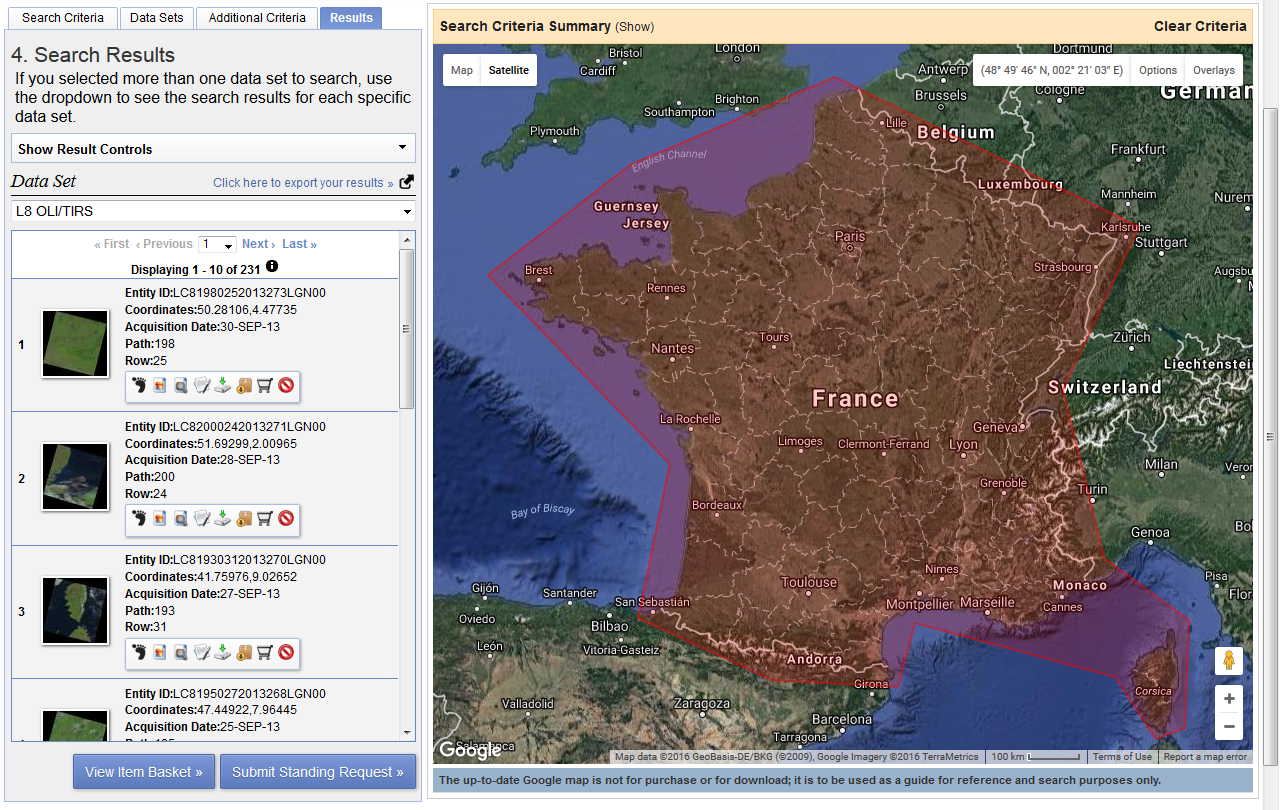
\includegraphics[scale=0.5]{images/france-selection.png}
\end{center}
% \caption{Polygone de sélection des scènes \begin{itshape}Landsat-8\end{itshape} pour la France sur l'interface du site de l'$USGS$}
\label{selection_france}
\end{figure}

Cette période correspond à l'année des valeurs de densité de population à notre disposition (et que nous présenterons plus tard) pour l'ensemble des communes de France.\\
La période de Mai à Septembre est la plus courte permettant de couvrir tout le territoire métroplitain tout en conservant une occupation
nuageuse inférieure à 20\%.
Nous obtenons ainsi 70 scènes \begin{itshape}Landsat-8\end{itshape} chacune correspondant à un couple $path$,$row$ unique.\\
Les figures \ref{cloud1},\ref{cloud3},\ref{cloud4} et \ref{cloud5} montrent des miniatures couleurs des 4 scènes parmi les 70, ayant une couverture 
nuageuse supérieure à 10\%.

\begin{figure}[H]
\begin{center}
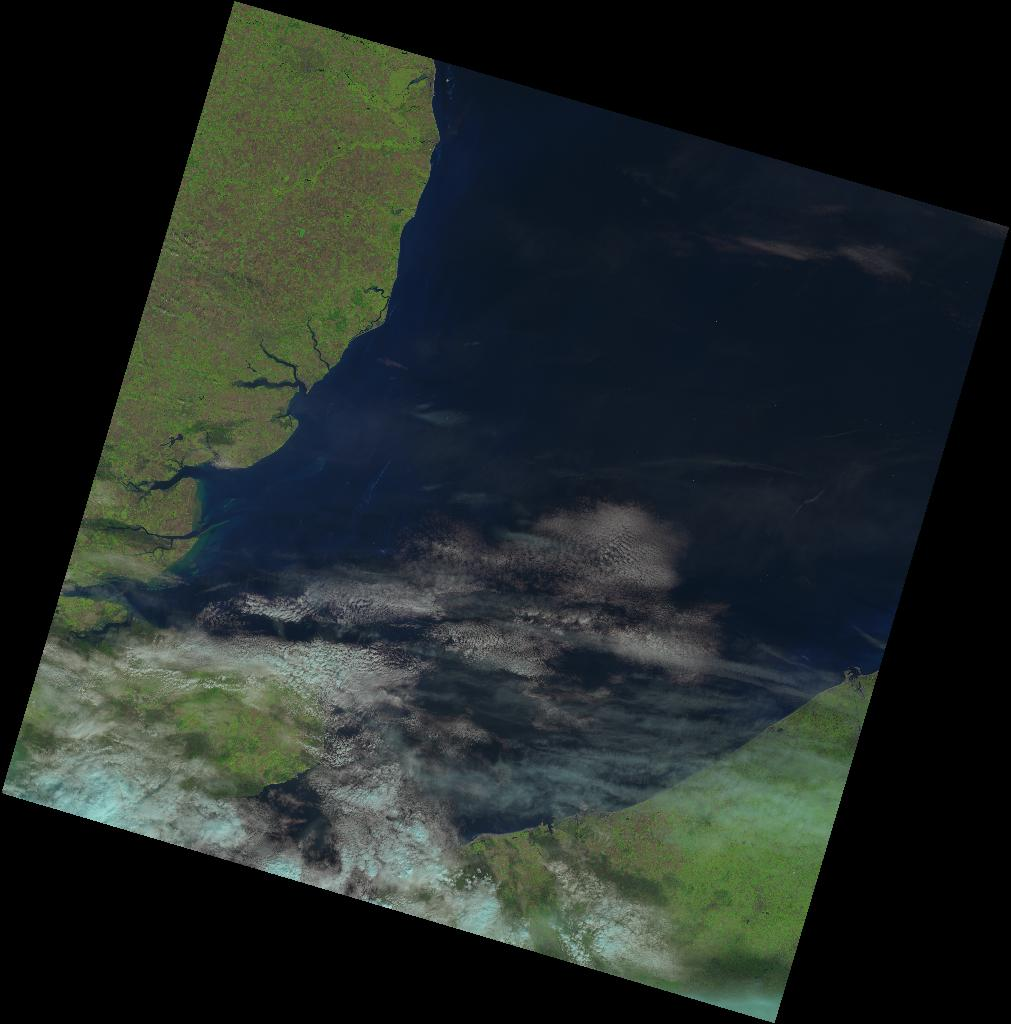
\includegraphics[scale=0.18]{images/LC82000242013271LGN00.jpg}
\end{center}
%\caption{Miniature couleur en projection Web Mercator (EPSG:3857) de la zone $200$,$024$ (region Nord-Pas-de-Calais) - couverture nuageuse de 20.00\% }
\label{cloud1}
\end{figure}

\begin{figure}[H]
\begin{center}
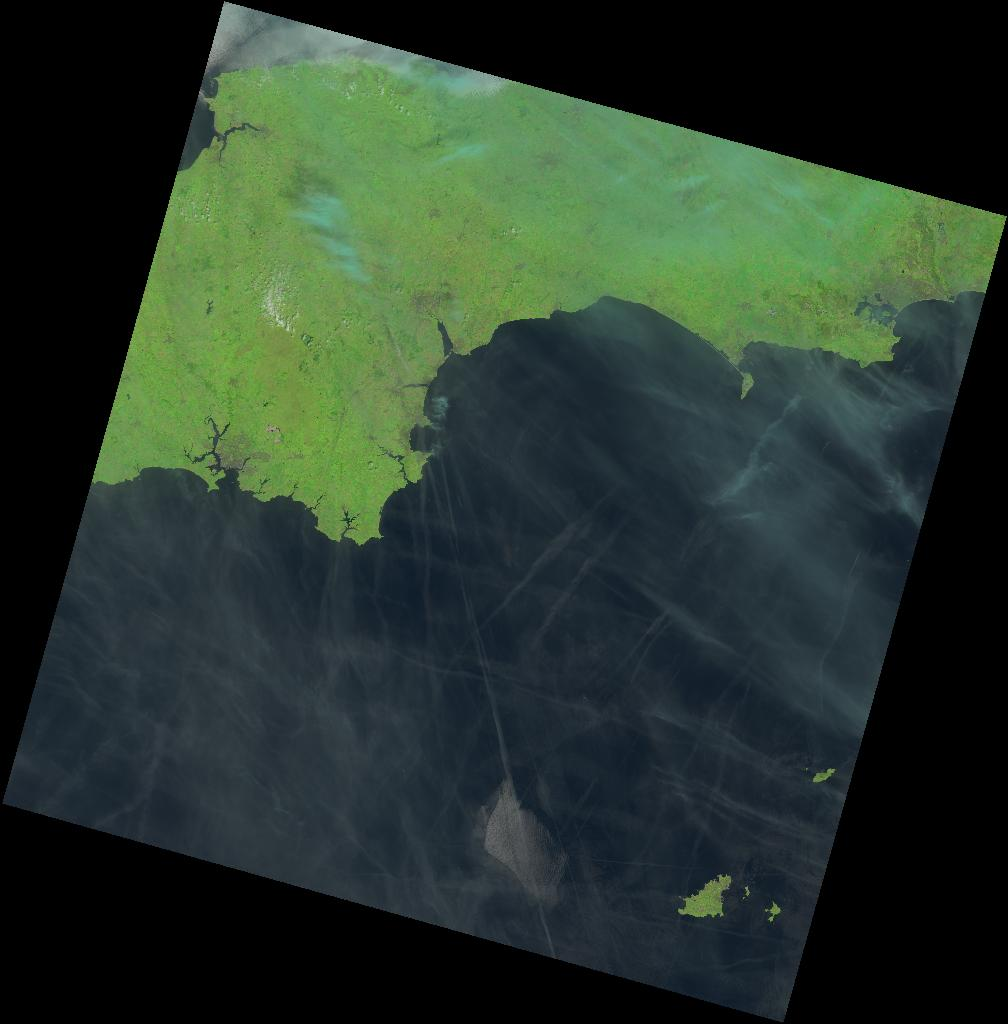
\includegraphics[scale=0.18]{images/LC82030252013196LGN00.jpg}
\end{center}
%\caption{Miniature couleur en projection Web Mercator (EPSG:3857) de la zone $203$,$025$ (région des îles anglo-normandes) - couverture nuageuse de 18.30\%}
\label{cloud3}
\end{figure}

\begin{figure}[H]
\begin{center}
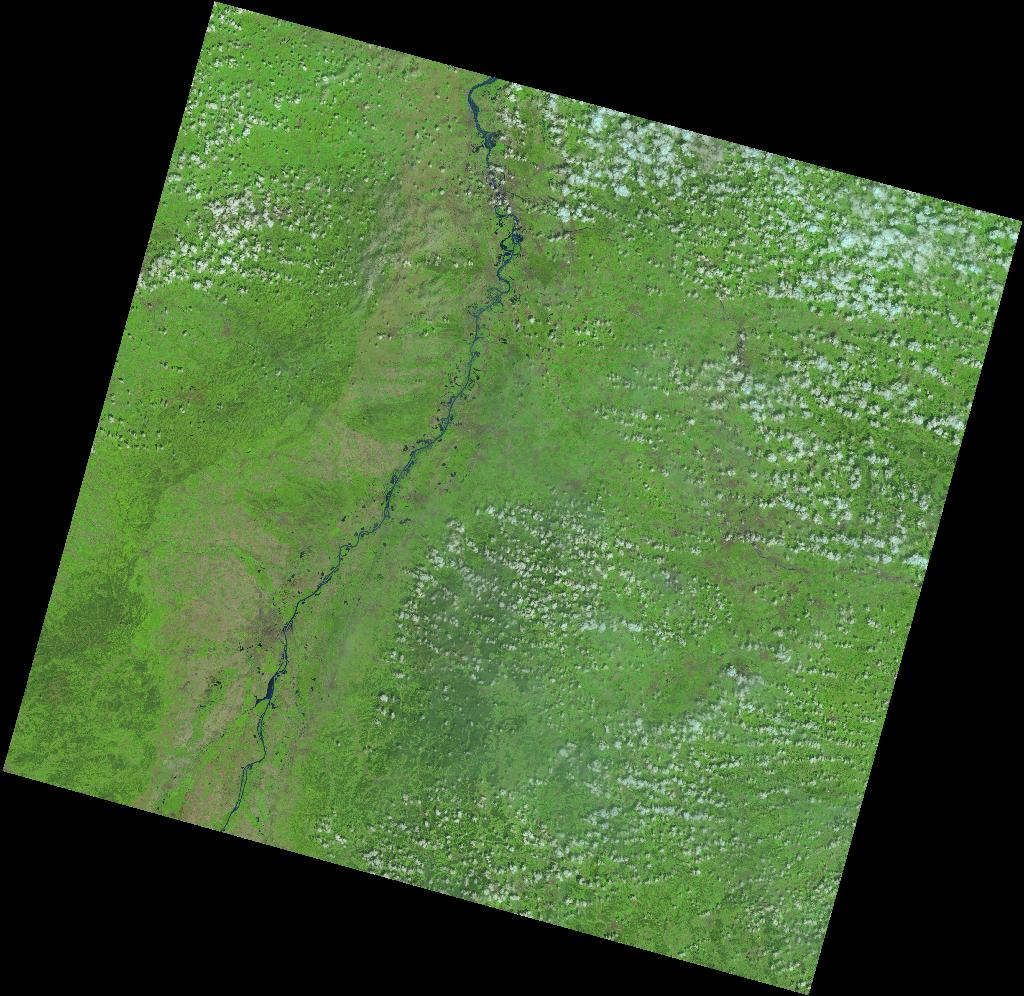
\includegraphics[scale=0.18]{images/LC81950262013156LGN00.jpg}
\end{center}
%\caption{Miniature couleur en projection Web Mercator (EPSG:3857) de la zone $195$,$026$ (poînte strasbourgeoise) - couverture nuageuse de 13.00\%}
\label{cloud4}
\end{figure}

\begin{figure}[H]
\begin{center}
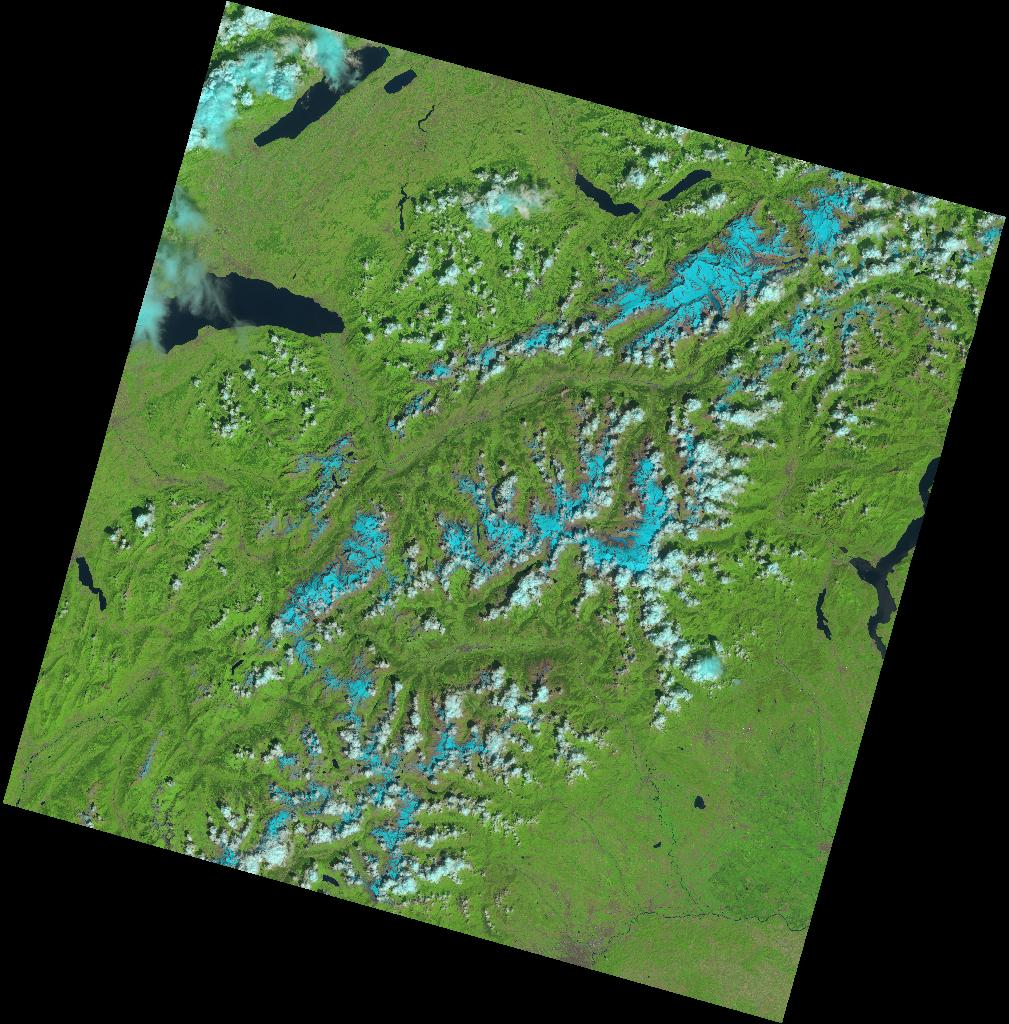
\includegraphics[scale=0.18]{images/LC81950282013204LGN00.jpg}
\end{center}
%\caption{Miniature couleur en projection Web Mercator (EPSG:3857) de la zone $203$,$028$ (frontière franco-italo-suisse) - couverture nuageuse de 12.60\%}
\label{cloud5}
\end{figure}

On voit donc que les scènes ayant une forte couverture nuageuse sont :
\begin{description}
\item[-] soit des scènes contenant beaucoup de domaine maritime
\item[-] soit des scènes limitrophes de pays voisins. 
\end{description}
La présence de nuage devrait donc avoir globalement une faible impacte sur le $NDVI$ des communes françaises.\\

la figure \ref{couverture} présente toutes les scènes après projection en Web Mercator (EPSG:3857). En effet, les images sont dites géoréférencées, c'est le 
sujet du chapître suivant.

\begin{figure}[H]
\begin{center}
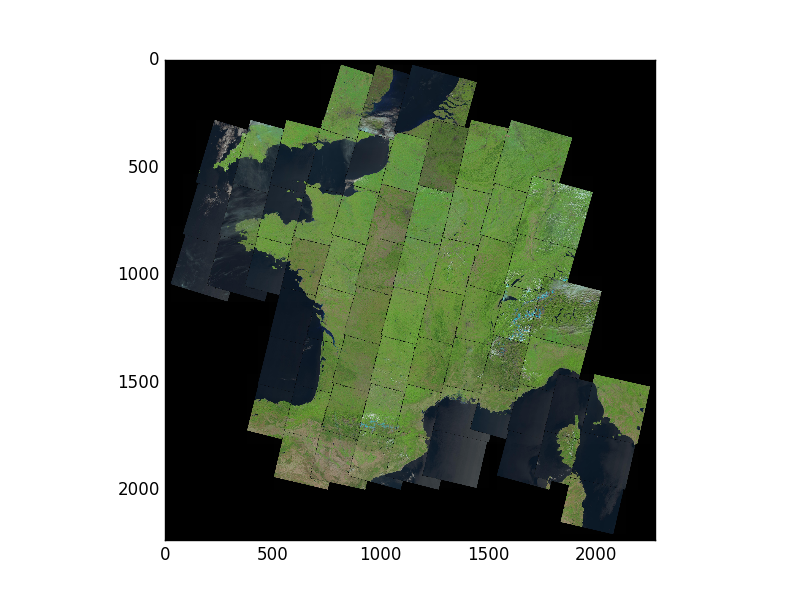
\includegraphics[scale=0.7]{images/france-covering.png}
\end{center}
\caption{Concaténation des 70 scènes Lansat-8 après projection en Web Mercator (EPSG:3857)}
\label{couverture}
\end{figure}


\chapter{Géoréférencement d'images aériennes}
\section{Principe}\label{principe_geo}

Concrètement le géoréférencement consiste à donner aux points 
d'une image rectangulaire de prise de vue aérienne, des coordonnées géographiques dans un certain système de coordonnées. 
En effet, un point de l'image est simplement répéré par ses coordonnées de ligne et de colonne mais n'a aucune caractéristique
géographique.\\
Dans le cas de Landsat-8, ces coordonnées sont fournies dans le système \begin{itshape}UTM Mercator\end{itshape}. Et nous allons dans ce chapître, 
vérifier si le géoréférencement de ces images est suffisamment précis\\

Une méthode simple pour le géoréférencement d'une image dans un certain système de coordonnées, nécessite la connaissance 
des coordonnées d'un 
certain nombre de points de l'image dans ce système de coordonnées, ce sont les \begin{itshape}points d'amers\end{itshape}.
A partir de ces points, une transformation d'un certain ordre est appliquée aux autres points de l'image afin de leur attribuer 
des coordonnées dans ce système.\\

\section{Les systèmes de géoréférencement}

Il en existe une multitude dont le nom est codifié par l'\begin{itshape}European Petroleum Survey Group\end{itshape} depuis 1985.\\
A titre d'exemple, l'$IGN$ (\begin{itshape}Institut Géographique National\end{itshape}) géoréférence ces images via plusieurs
systèmes de géoréférencement possibles dont:\\

\begin{itemize}

\item[-] \begin{itshape}NTF 93/Lambert 93\end{itshape} dont le code est \begin{itshape}EPSG:2154\end{itshape}.\\
\item[-] \begin{itshape}NTF Paris/Lambert zone II étendu\end{itshape} dont le code est \begin{itshape}EPSG:27572\end{itshape}.\\
 
\end{itemize}

Les images du satellite \begin{itshape}Landsat-8\end{itshape} sont géoréférencées dans le système 
\begin{itshape}WGS84/Mercator\end{itshape} dont le code $EPSG$ dépend
de la zone $UTM$ (\begin{itshape}Universe Transverse Mercator\end{itshape}) où l'on se situe dans le globe 
(par exemple \begin{itshape}EPSG:32631\end{itshape} pour la zone \begin{itshape}UTM\end{itshape} $31N$ contenant la commune de
 \begin{itshape}Thonon-Les-Bains\end{itshape}).\\ 
Dans la section qui suit, nous proposons une méthode pour vérifier la fiabilité du géoréférencement
 des images du satellite \begin{itshape}Landsat-8\end{itshape}.
 
\section{Géoréférencement des images Landsat-8}

Le site de l'$USGS$ (\begin{itshape}U.S. Geological Survey\end{itshape}) \cite{landsat8} qui met à disposition les images
satellitaires de \begin{itshape}Landsat-8\end{itshape}, ne précise pas la méthode utilisée pour leur géoréférencement.
Mais on peut toutefois vérifier sa fiabilité en comparant une image de ce satellite avec une image de 
l'$IGN$.\\
En effet, il suffirait de récupérer une image d'une certaine zone au format \begin{itshape}GeoTIFF\end{itshape}, 
donc géoréférencé, de l'$IGN$ et de la superposer
à une image \begin{itshape}Landsat-8\end{itshape} contenant la même zone. Toutefois, le géoréférencement de l'image $IGN$ étant différent
de celui de l'image \begin{itshape}Landsat-8\end{itshape}, il faudrait afficher la première dans le géoréférencement de la seconde.\\
Seulement, le site de l'$IGN$ ne propose des images géoréférencées qu'à l'achat, mais nous pouvons contourner cela en récupérant une 
carte non géoréférencé, qu'on géoréférencerait ensuite via un logiciel pour les Systèmes d'Information Géopgraphique ($SIG$), 
$QGIS$ en l'occurence.

\subsection{Création d'une carte géoréférencée de l'IGN}

Le portail de l'IGN \cite{ign-portail} permet de parcourir le globe en affichant instantanément les coordonnées des points dans 
plusieurs systèmes de coordonnées possibles. La figure \ref{ign-portail} montre l'interface du portail affichant la commune de
\begin{itshape}Thonon-Les-Bains\end{itshape} en coordonnées \begin{itshape}NTF 93/Lambert 93\end{itshape}.

\begin{figure}[H]
\begin{center}
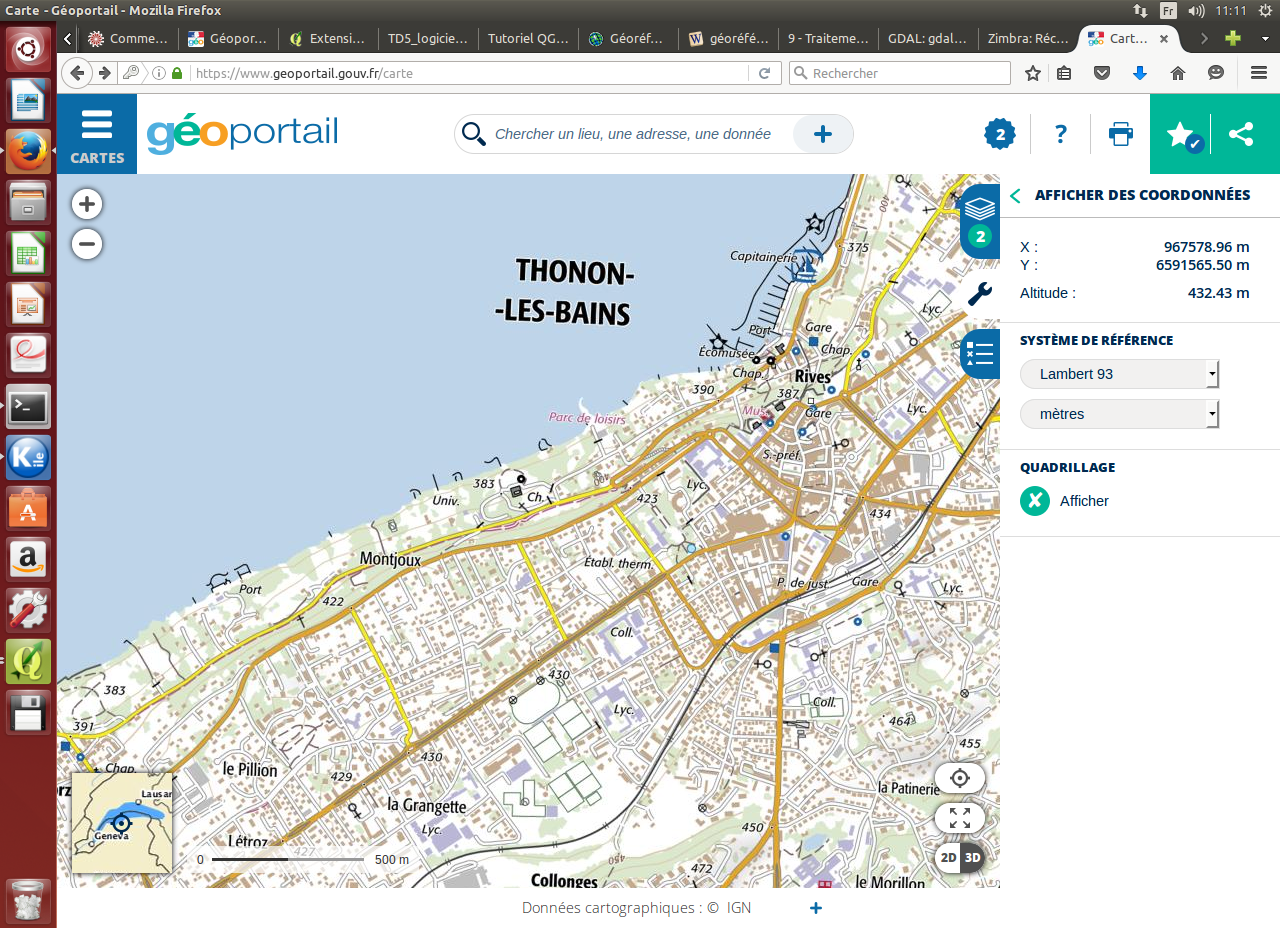
\includegraphics[scale=0.3]{images/georeferencing/ign-portail-Thonon.png}
\end{center}
\caption{Portail de l'$IGN$ - commune de Thonon-Les-Bains en coordonnées NTF93/Lambert93 \cite{ign-portail}}
\label{ign-portail}
\end{figure}

La manipulation consiste à prendre un snapshot du portail pour cette zone, en y inscrivant au préalable les coordonnées de 
plusieurs points via l'outil de marquage et d'annotation du portail. La figure \ref{ign-points} montre ainsi six points 
dont on a indiqué les coordonnées en \begin{itshape}NTF 93/Lambert 93\end{itshape}. Ces points vont jouer le rôle des 
\begin{itshape}points d'amers\end{itshape} décrits plus haut dans le principe de géoréférencement \ref{principe_geo}.

\begin{figure}[H]
\begin{center}
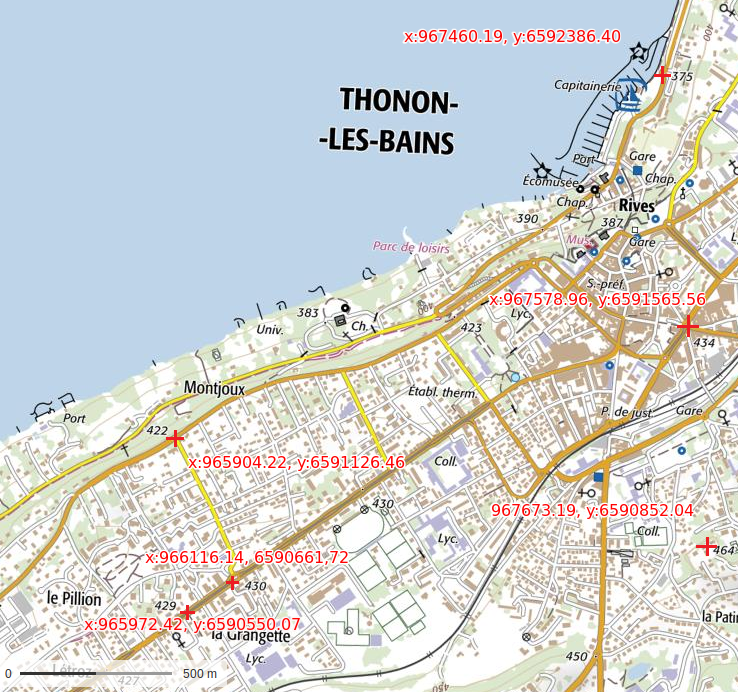
\includegraphics[scale=0.5]{images/georeferencing/ign-points-Thonon.png}
\end{center}
\caption{Carte non-géoréférencé de l'$IGN$ - commune de Thonon-Les-Bains et six points de contr\^{o}le en coordonnées NTF93/Lambert93}
\label{ign-points}
\end{figure}

Le logiciel libre $QGIS$ \cite{QGIS_software} permet de géoréférencer une image ou une carte dans le même système de coordonnées que des points de
contr\^{o}le préalablement renseignés dans l'outil.\\
Pour commencer, il faut ouvrir un projet dans la fen\^{e}tre principale et renseigner le système de projection dans lequel on souhaite visualiser
les images géoréférencées (on parle de \begin{itshape}raster\end{itshape}). On choisit ici le système de projection
\begin{itshape}EPSG:32631\end{itshape} car c'est celui dans lequel les images \begin{itshape}Landsat-8\end{itshape} (dans la zone $UTM$ 
de \begin{itshape}Thonon-Les-Bains\end{itshape}) sont projetées et
sur lequel on projetera notre carte IGN une fois géoréférencée, pour comparaison.\\
La figure \ref{qgis-projet} montre la manipulation dans les propriétés du projet.

\begin{figure}[H]
\begin{center}
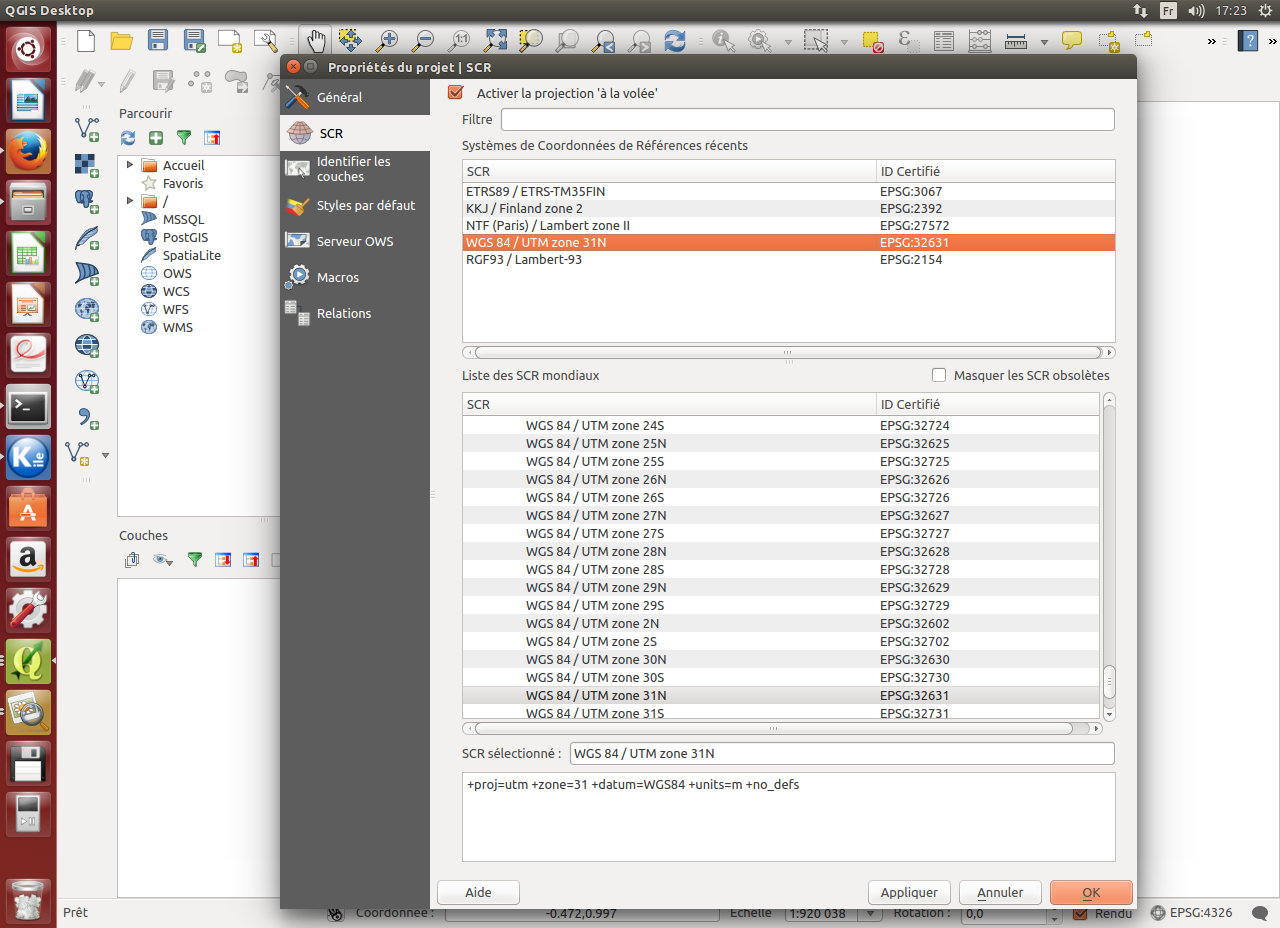
\includegraphics[scale=0.3]{images/georeferencing/qgis-projet.png}
\end{center}
\caption{Projet $QGIS$ et système de projection}
\label{qgis-projet}
\end{figure}

Ensuite, via l'onglet \og Raster > Géoréférencer > Géoréférencer\fg{}, on ouvre 
une nouvelle fen\^{e}tre dédiée au géoréférencement à partir de laquelle on charge notre carte \ref{qgis-georef} 
(onglet \og Ajouter un raster \fg{}).\\
L'outil demande alors de renseigner un système de projection pour le géoréférencement, on selectionne celui correspondant 
à nos points d'amers, soit \begin{itshape}NTF 93/Lambert 93\end{itshape} (\begin{itshape}EPSG:2154\end{itshape}).

\begin{figure}[H]
\begin{center}
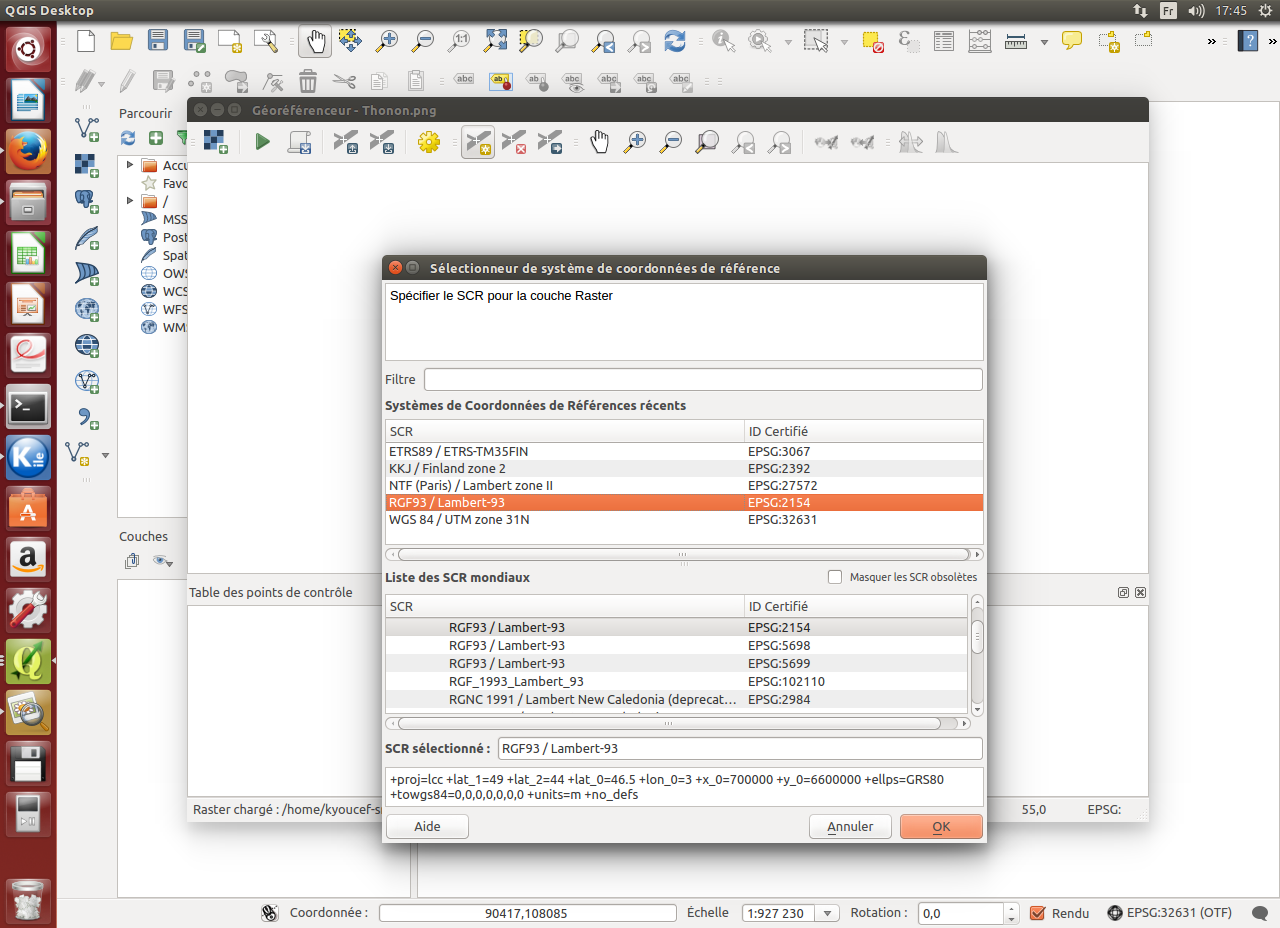
\includegraphics[scale=0.3]{images/georeferencing/qgis-georef.png}
\end{center}
\caption{Projet $QGIS$ et chargement d'une image non-géoréférencé pour géoréférencement}
\label{qgis-georef}
\end{figure}

Une fois le snapshot chargé, on renseigne les points de contr\^{o}le correspondant aux croix rouges sur le snapshot via l'onglet 
\og Ajouter un point \fg{}, dans la fenêtre de géoréférencement. On ajoute tour à tour les six points en renseignant
les coordonnées des points. La figure \ref{qgis-points} montre ainsi la fen\^{e}tre de géoréférencement contenant le snapshot 
et le tableau des points de contr\^{o}le en bas.

\begin{figure}[H]
\begin{center}
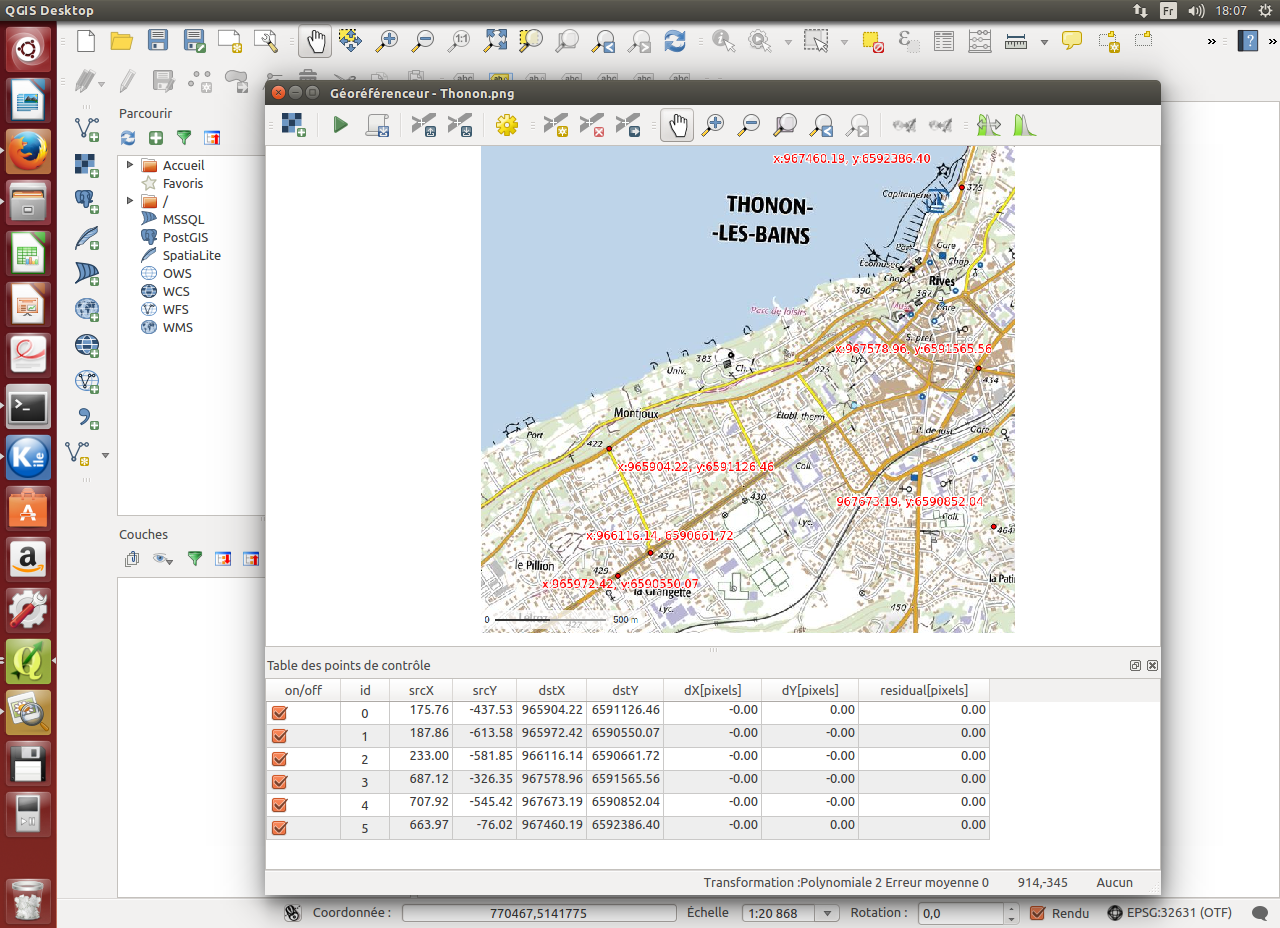
\includegraphics[scale=0.3]{images/georeferencing/qgis-points.png}
\end{center}
\caption{Projet $QGIS$ et renseignement des points de contr\^{o}le dans la fen\^{e}tre de géoréférencement}
\label{qgis-points}
\end{figure}

Maintenant que les points de renseignement sont donnés, on va définir la transformation à appliquer. Pour cela, on ouvre l'onglet
 \og Paramètres > Tranformation \fg{}, qu'on renseigne comme dans la figure \ref{qgis-transformation}. Par ordre, 
on renseigne le type de transformation, ici polynomiale du second degré. En effet, avec six points d'amers, on peut se permettre
une transformation non linéaire d'ordre 2 en vertu de la formule \cite{Nicolas:2014}:

\[P\ge\frac{(L+1)(L+2)}{2}\]

où $L$ est le degré du polyn\^{o}me et $P$, le nombre de points d'amers nécessaires.\\
On renseigne aussi le type de réechantillonnage des pixels, afin d'affecter une valeur aux pixels qui n'en auront pas
après transformation. Et enfin, on renseigne le système de géoréférencement correspondant 
à nos points d'amers, soit \begin{itshape}NTF 93/Lambert 93\end{itshape} (\begin{itshape}EPSG:2154\end{itshape}). On peut aussi
 cocher la case \og charger dans QGIS lorsque terminé \fg{} afin d'avoir l'image géoréférencé directement
 projeté dans le système de coordonnées du projet (\begin{itshape}EPSG:32631\end{itshape}).

\begin{figure}[H]
\begin{center}
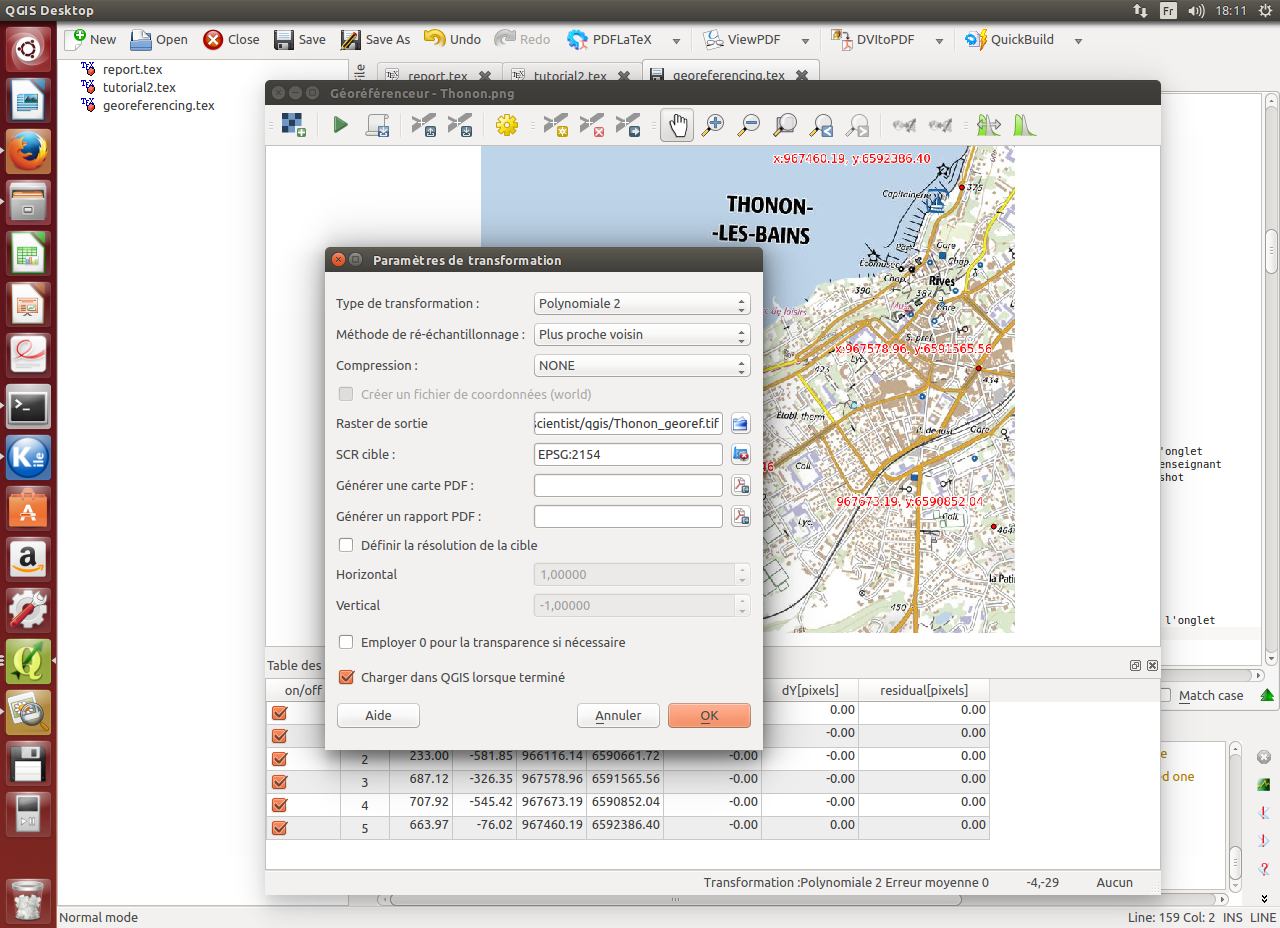
\includegraphics[scale=0.3]{images/georeferencing/qgis-transformation.png}
\end{center}
\caption{Projet $QGIS$ et renseignement de la transformation dans la fen\^{e}tre de géoréférencement}
\label{qgis-transformation}
\end{figure}

Il ne reste qu'à lancer la géoréférencement via la flèche verte dans la fen\^{e}tre de géoréférencement, cela va afficher
notre snapshot dans le système de coordonnées \begin{itshape}EPSG:32631\end{itshape} \ref{qgis-resultat}.

\begin{figure}[H]
\begin{center}
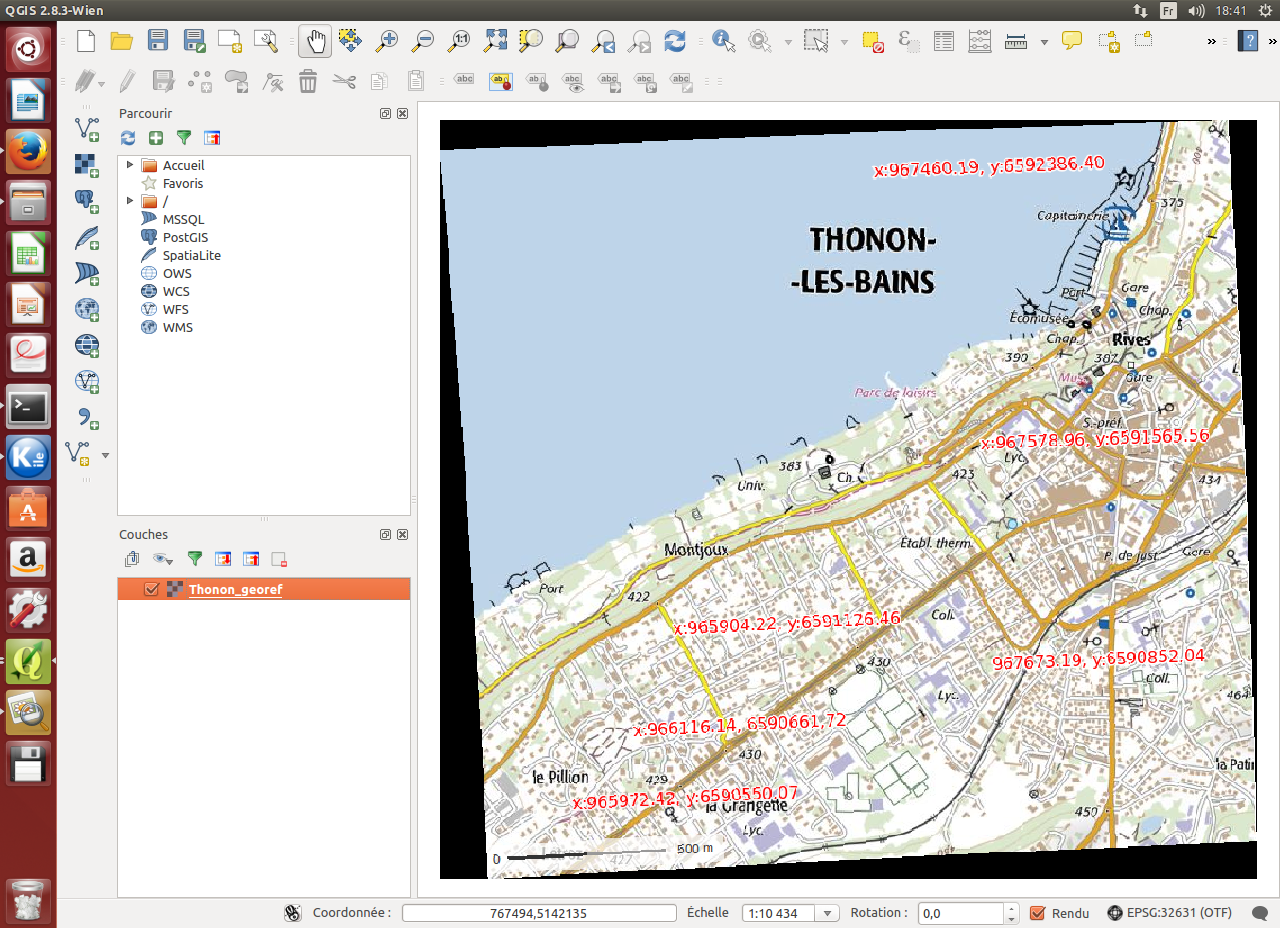
\includegraphics[scale=0.3]{images/georeferencing/qgis-resultat.png}
\end{center}
\caption{Projet $QGIS$ et affichage du raster géoéréférencé projeté dans la fen\^{e}tre principale}
\label{qgis-resultat}
\end{figure}

\subsection{Superposition d'un raster Landsat-8}

A présent que notre snapshot IGN est géoréférencé et projeté dans le système de coordonnées de \begin{itshape}Landsat-8\end{itshape}
(\begin{itshape}EPSG:32631\end{itshape}), on peut charger une image géoréférencé \begin{itshape}Landsat-8\end{itshape} contenant la 
commune de \begin{itshape}Thonon-Les-Bains\end{itshape}. Pour cela, on a téléchargé les bandes 2,3,4 correspondantes et formé l'image 
couleur  \ref{Thonon-landsat}. On peut vérifier que le système de géoréférencement de ces images est bien \begin{itshape}EPSG:32631\end{itshape} via la 
commande \begin{itshape}listgeo\end{itshape}:\\

\begin{center}
listgeo LC81960282016252LGN00\_B2.TIF
\end{center}

qui renvoit bien ($PCS$ pour \begin{itshape}Projection Coordinate System\end{itshape}) :\\

\begin{center}
PCS = 32631 (WGS 84 / UTM zone 31N)\\
\end{center}

\clearpage

\begin{figure}[H]
\begin{center}
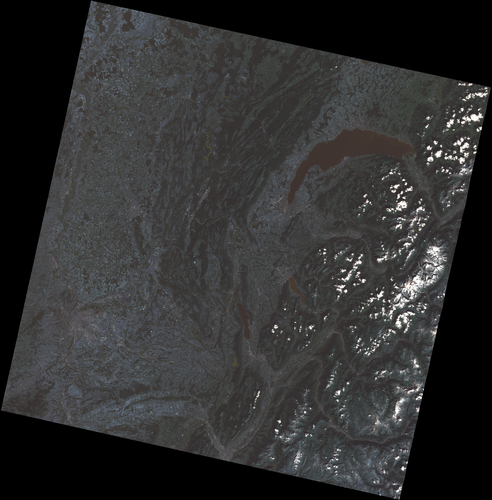
\includegraphics[scale=0.4]{images/georeferencing/Thonon_landsat.png}
\end{center}
\caption{Image couleur à partir d'images géoréférencées Landsat-8 contenant la commune de Thonon-Les-Bains}
\label{Thonon-landsat}
\end{figure}

On peut alors charger cette image dans la fenêtre principale $QGIS$ via l'onglet \og Couche > Ajouter une couche > Ajouter une couche 
raster \fg{}. On observe au final la superposition des deux rasters et dont on peut régler la transparence (sous-fen\^{e}tre \og couches \fg{}) 
dans la fen\^{e}tre principale $QGIS$) \ref{qgis_super}

\begin{figure}[H]
\begin{center}
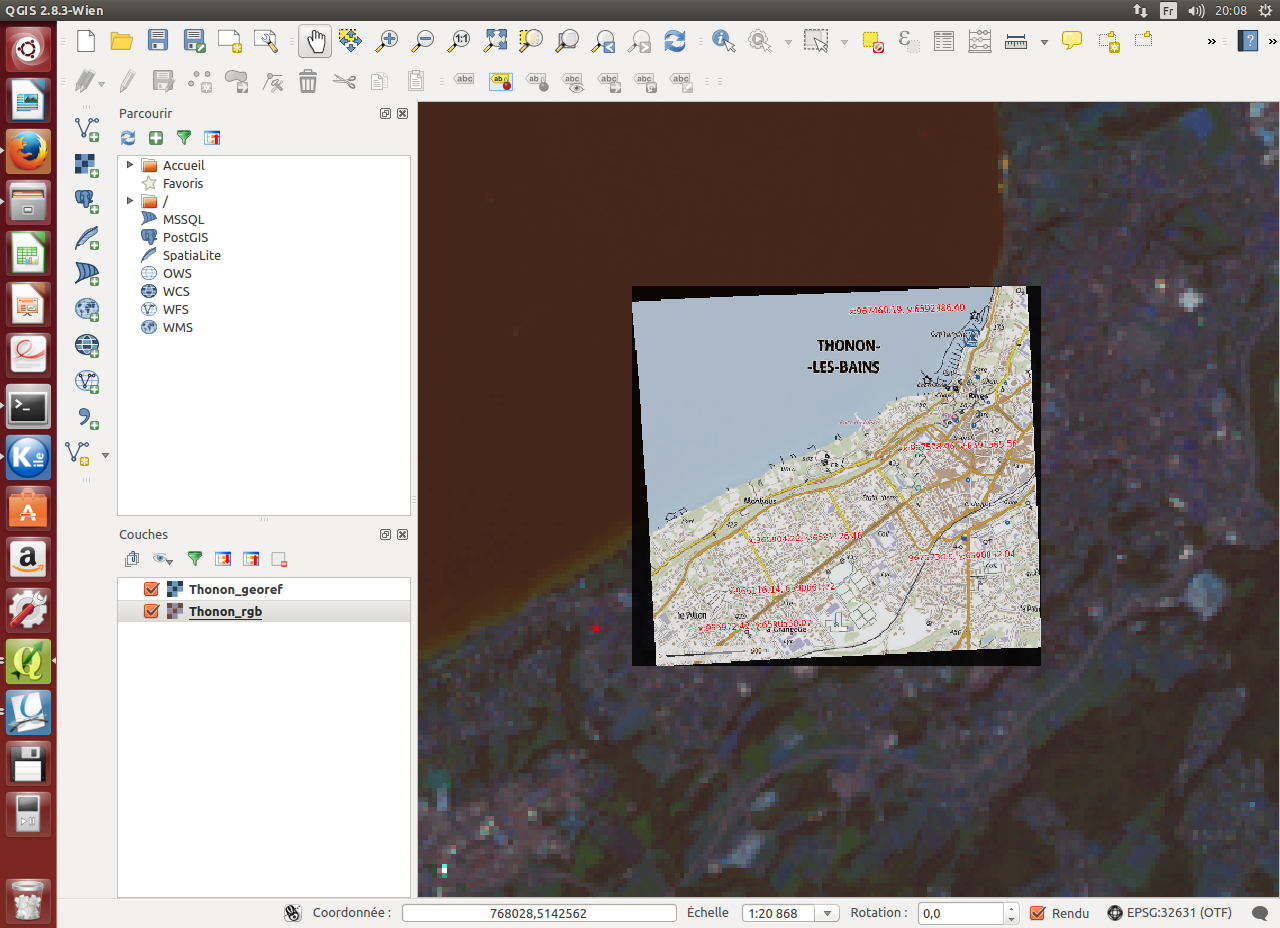
\includegraphics[scale=0.3]{images/georeferencing/qgis-superposition0.png}
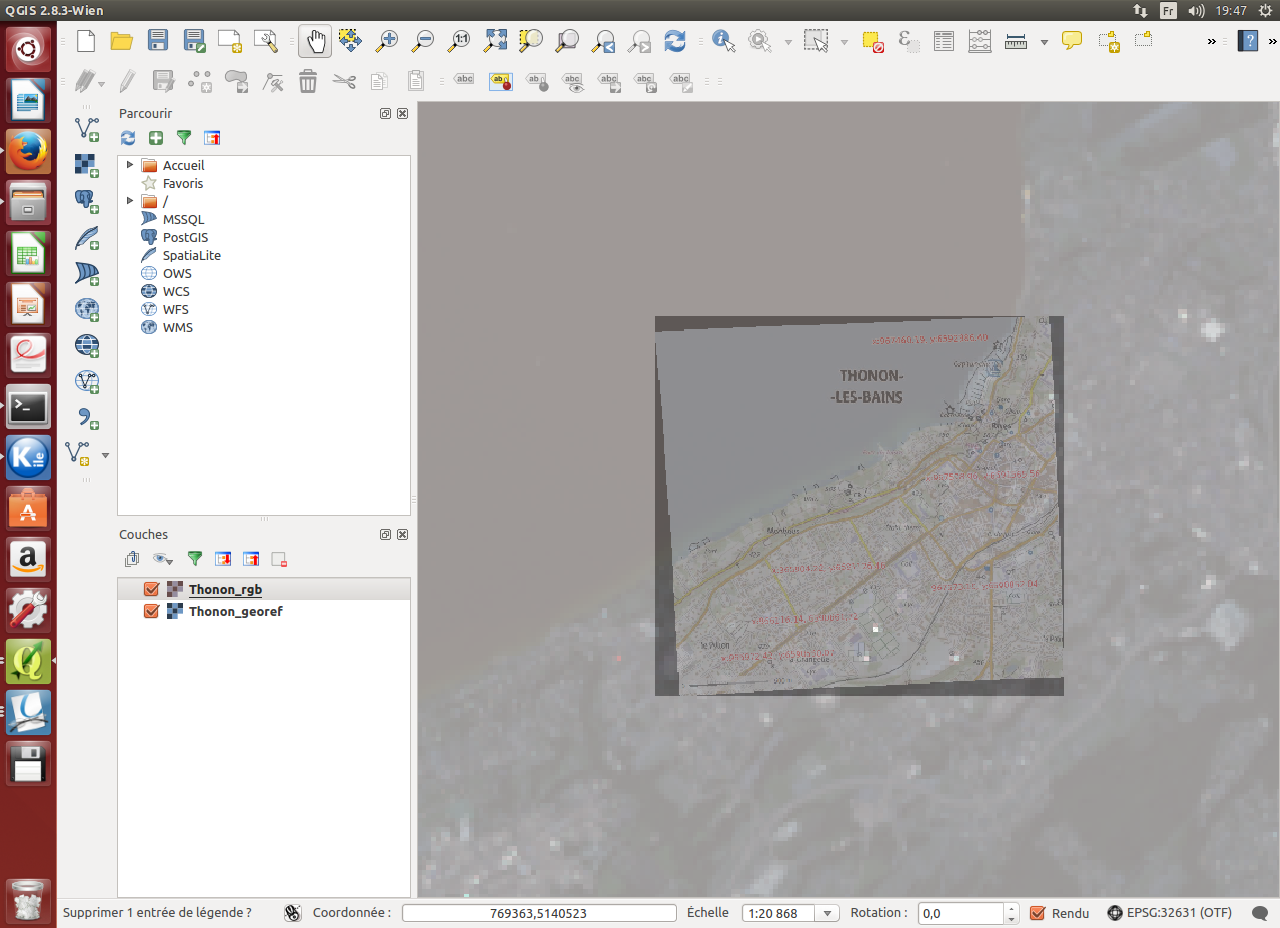
\includegraphics[scale=0.3]{images/georeferencing/qgis-superposition.png}
\end{center}
\caption{Projet $QGIS$ et superposition des rasters IGN et Landsat-8 géoréférencés en EPSG:32631 - commune de Thonon-Les-Bains}
\label{qgis_super}
\end{figure}

On constate une assez bonne superposition des deux rasters, le géoréférencement du satellite \begin{itshape}Landsat-8\end{itshape} peut
 donc \^{e}tre considéré comme convenable.

\chapter{Métadonnées des communes françaises}

\section{Géolocalisation, surface et population}

Cette section présente la manière dont sont récupérées les données de communes françaises. En effet, nous avons besoin pour chacune d'elle  :
\begin{itemize}
  \item des longitude et latitude, qu'on convertira en coordonnées géographiques (\begin{itshape}Web Mercator\end{itshape}) afin de repérer précisemment la commune.
  \item de la surface, qui nous permettra d'identifier un périmètre carré de même surface, autour de la commune.
  \item de sa population, ou de sa densité directement.
\end{itemize}

Les données de nom, de population et de surface de plus de 36000 comunes sont obtenues dans le fichier de recensement de l'INSEE de 2013 \cite{insee_pop2013}.\\
Les données de géolocation (latitude et longitude) sont obtenues via l'API Python \begin{itshape}Geopy\end{itshape} \cite{geopy}. Elle permet d'instancier 
le géolocalisateur de Google et de procéder à des requêtes pour chacune des communes.\\

Ainsi, on obtient un tableau des métadonnées necessaires à la labélisation de nos communes en vue d'une classification supervisée \ref{tab_meta}.

\begin{table}[H]
\begin{center}
\begin{adjustbox}{max width=\textwidth}
{
\begin{tabular}{|c|c|c|c|c|}
\hline 
nom & latitude (degrés) & longitude (degrés) & surface (km\textsuperscript{2}) & densité (habs/km\textsuperscript{2}) \\
\hline
Ozan & 46.391534 & 4.915265 & 6.6 & 98.3\\
\hline 
Cormoranche-sur-Sa\^{o}ne & 46.240532 & 4.830863 & 9 & 118.9\\
\hline 
Paris & 48.856614 & 2.352222 & 105.4 & 21153.9\\
\hline
Lyon & 45.764043 & 4.835659 & 47.87 & 10117.0\\
\hline
Tours & 47.394144 & 0.68484 & 34.67 & 3888.2\\
\hline
Besancon & 47.237829 & 6.024054 & 65.05 & 1797.9\\
\hline 
... & ... & ... & ... & ... \\
\hline
\end{tabular}
}
\end{adjustbox}
\end{center}
\caption{Métadonnées liées aux communes françaises}
\label{tab_meta}
\end{table}

Afin de nous rapporter à un problème de classification pour la prédiction de la densité, nous allons labelliser nos communes par catégorisation de leur distribution.
Pour cela, on va rechercher le meilleur découpage de cette distribution par la méthode d'Otsu à multi-seuillage. Elle permet de déterminer le nombre de seuils et leurs
 valeurs, qui permettent de minimiser la variance intra catégories et maximiser la variance inter catégories. C'est l'objet de la section qui suit.

\section{Catégorisation de la densité}\label{cat}

Il s'agit de découper l'intervalle de densité en une partition d'intervalles. La multi-binarisation d'Otsu permet de créer une telle partition en
minimisant la variance au sein de chaque partition, tout en maximisant la variance inter-partition.\\
La figure \ref{densite_histo} présente l'histogramme de densité de nos échantillons :

\begin{figure}[H]
\begin{center}
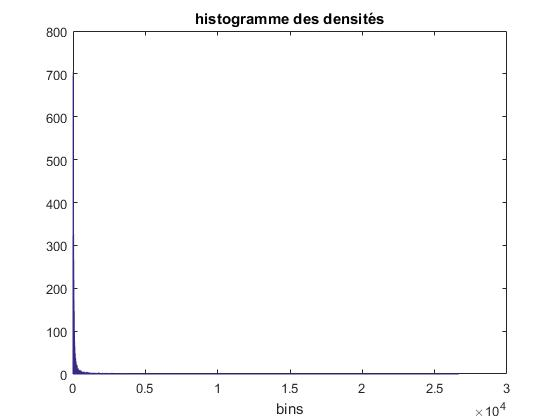
\includegraphics[scale=0.5]{images/densite_histo.jpg}
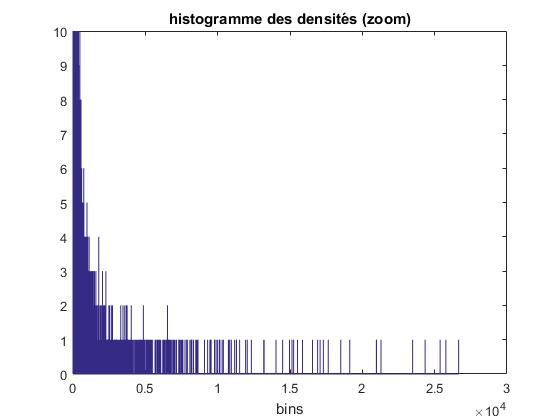
\includegraphics[scale=0.5]{images/densite_histo_zoom.jpg}
\end{center}
\caption{Histogramme des densités et son zoom}
\label{densite_histo}
\end{figure}

On applique alors la méthode d'Otsu ($Matlab$) sur l'histogramme pour différentes valeurs en nombre de catégories (ou nombre de clusters si on voit la méthode comme
une méthode de segmentation). On obtient à chaque fois un score reflétant la compacité des catégories créées. On obtient un score maximal pour un nombre de catégories de 6.\\
La figure \ref{densite_histo_otsu} montre graphiquement les 5 seuils obtenus pour la segmentation  à 6 catégories.

\begin{figure}[H]
\begin{center}
  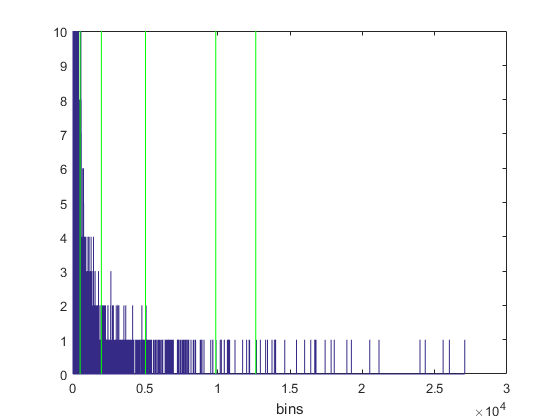
\includegraphics[scale=0.7]{images/labels/densite_histo_otsu_zoom.png}
\end{center}
\caption{Histogramme de densité (habs/km\textsuperscript{2})}
\label{densite_histo_otsu}
\end{figure}

On obtient ainsi les six catégories suivantes \ref{tab_meta_categorie}.

\begin{table}[H]
\begin{center}
\begin{adjustbox}{max width=\textwidth}
{
\begin{tabular}{|c|c|}
    \hline 
    \textbf{catégorie 1} & densité comprise entre 0 et 500 habs/km\textsuperscript{2}\\
    \hline
    \textbf{catégorie 2} & densité comprise entre 500 et habs/km\textsuperscript{2}\\
    \hline
    \textbf{catégorie 3} & densité comprise entre 2000 et 5000 habs/km\textsuperscript{2}\\
    \hline
    \textbf{catégorie 4} & densité comprise entre 5000 et 10000 habs/km\textsuperscript{2}\\
    \hline
    \textbf{catégorie 5} & densité comprise entre 10000 et 13000 habs/km\textsuperscript{2}\\
    \hline
    \textbf{catégorie 6} & densité supérieure à 13000 habs/km\textsuperscript{2}\\
    \hline
\end{tabular}
}
\end{adjustbox}
\end{center}
\caption{Catégorisation de la densité des communes françaises}
\label{tab_meta_categorie}
\end{table}

D'où notre tableau final des métadonnées des communes françaises \ref{tab_meta_cat}

\begin{table}[H]
\begin{center}
\begin{adjustbox}{max width=\textwidth}
{
\begin{tabular}{|c|c|c|c|c|c|}
\hline 
nom & latitude (degrés) & longitude (degrés) & surface (km\textsuperscript{2}) & densité (habs/km\textsuperscript{2}) & \textbf{densité (categories)}\\
\hline
Ozan & 46.391534 & 4.915265 & 6.6 & 98.3 & 1\\
\hline 
Cormoranche-sur-saone & 46.240532 & 4.830863 & 9 & 118.9 & 1\\
\hline 
Paris & 48.856614 & 2.352222 & 105.4 & 21153.9 & 6\\
\hline
Lyon & 45.764043 & 4.835659 & 47.87 & 10117.0 & 5\\
\hline
Tours & 47.394144 & 0.68484 & 34.67 & 3888.2 & 3\\
\hline
Besancon & 47.237829 & 6.024054 & 65.05 & 1797.9 & 1\\
\hline 
... & ... & ... & ... & ... & ...\\
\hline
\end{tabular}
}
\end{adjustbox}
\end{center}
\caption{Métadonnées liées aux communes françaises après labelisation}
\label{tab_meta_cat}
\end{table}


\chapter{Extraction de l'histogramme de NDVI}

\section{Calcul de l'indice de végétation par différence normalisée (NDVI)}

Cet indice est calculé à partir des canaux
rouge ($R$) et proche-infrarouge ($PIR$) via la formule : 

\[NDVI=\frac{PIR-R}{PIR+R}\]

Typiquement :
\begin{description}
 \item[-] L'eau, la neige et les nuages refléchissent plus dans le rouge que dans le proche-infrarouge, soit un $NDVI$ négatif\\
 \item[-] Les sols nus réfléchissent tout autant dans les deux bandes d'où un NDVI nul\\
 \item[-] En revanche, les sols revétus de végétaux refléchissent bien plus dans le proche infra-rouge, ce qui donne un $NDVI$ positif, et d'autant
plus positif que la végétation est dense.\\
\end{description}

Afin de calculer un tel indice sur les images \begin{itshape}Landsat-8\end{itshape}, nous utilisons les bandes géoréférencées $4$ et $5$ 
qui jouent respectivement les r\^oles du rouge (\begin{itshape}0.85-0.88nm\end{itshape}) et du proche-infrarouge (\begin{itshape}0.64-0.67nm\end{itshape}).\\
la librairie $gdal$ \cite{dans-gdal} sur $python$ nous permet d'effectuer l'opération de différence normalisée sur des rasters pour produire une image de $NDVI$ géoréférencée ($GeoTIFF$).

\begin{figure}[H]
\centerline{
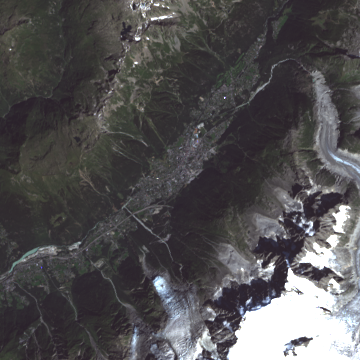
\includegraphics[scale=0.45]{../3_ndvi/images/Chamonix/08_rgb.png}
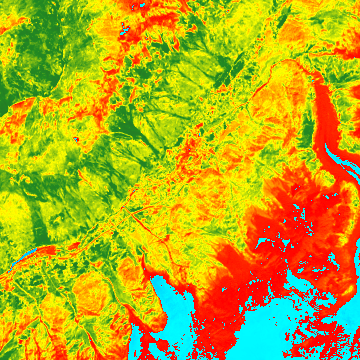
\includegraphics[scale=0.45]{../3_ndvi/images/Chamonix/08_ndvi.png}
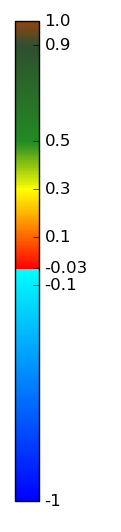
\includegraphics[scale=0.4]{../3_ndvi/images/colormap.png}
}
\begin{center}
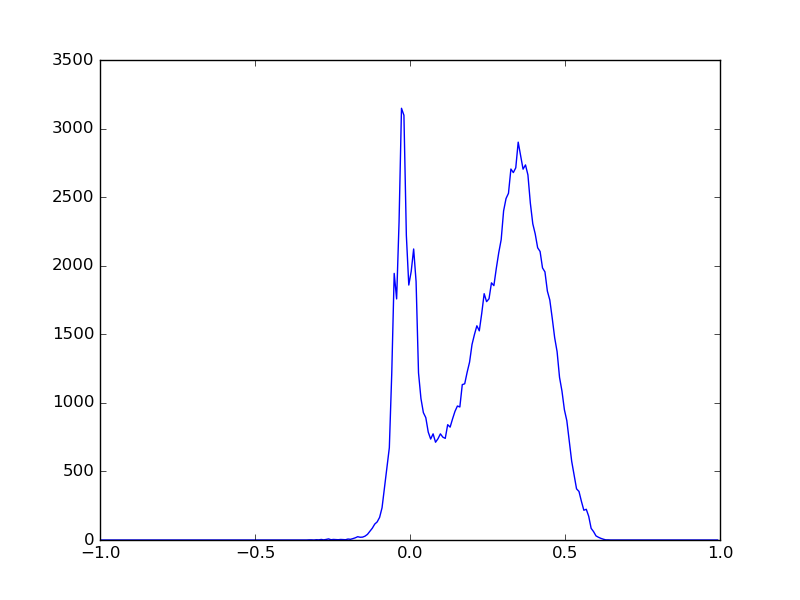
\includegraphics[scale=0.45]{../3_ndvi/images/Chamonix/08_ndvi_histo.png}
\end{center}
\caption{Image couleur, image $NDVI$ et histogramme de $NDVI$ pour la commune de $Chamonix-Mont-Blanc$ sur un périmètre de $116$km\textsuperscript{2} au mois d'$Aout$}
\label{chamonix_ndvi}
\end{figure}

La figure \ref{chamonix_ndvi} montre un $NDVI$ négatif au sud de la commune de Chamonix, ce qui correspond au glaciers du \begin{itshape}Mont-Blanc\end{itshape}\\

\clearpage 

\begin{figure}[H]
\centerline{
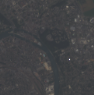
\includegraphics[scale=0.045]{../3_ndvi/images/Manaus/07_rgb.png}
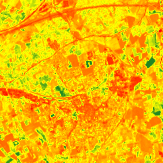
\includegraphics[scale=0.045]{../3_ndvi/images/Manaus/07_ndvi.png}
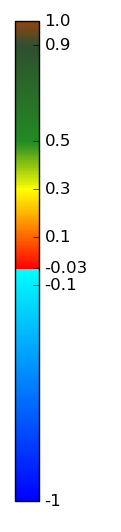
\includegraphics[scale=0.4]{../3_ndvi/images/colormap.png}
}
\begin{center}
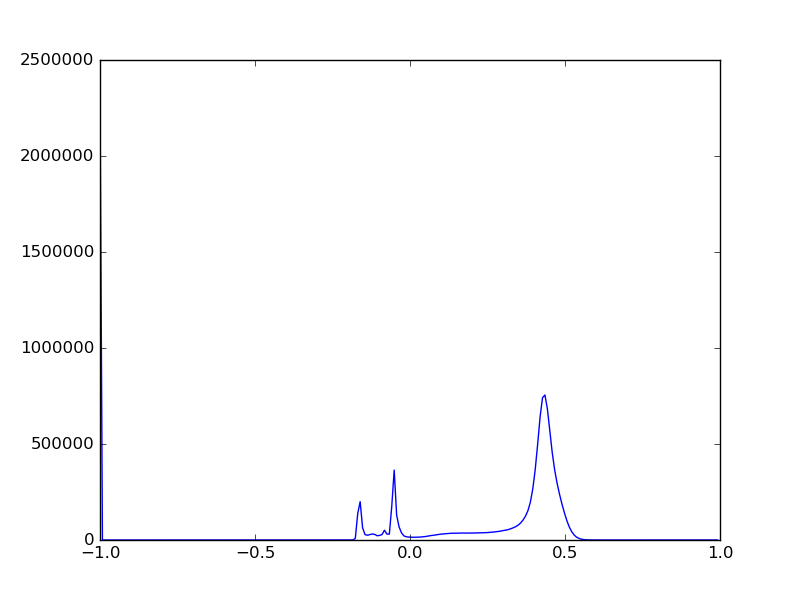
\includegraphics[scale=0.45]{../3_ndvi/images/Manaus/07_ndvi_histo.png}
\end{center}
\caption{Image couleur, image $NDVI$ et histogramme de $NDVI$ pour la ville de $Manaus$ ($Bresil$) sur un périmètre de $11000$km\textsuperscript{2} au mois de $Juillet$}
\label{manaus_ndvi}
\end{figure}

La figure \ref{manaus_ndvi} montre un $NDVI$ supérieur à $0.5$ autour de la ville de Manaus au Brésil, ce qui correspond à la végétation dense de la for\^et amazonienne. Le fleuve
du \begin{itshape}Rio Negro\end{itshape} apparait lui en négatif.\\

\clearpage

\begin{figure}[H]
\centerline{
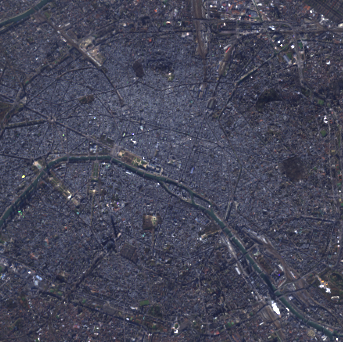
\includegraphics[scale=0.45]{../3_ndvi/images/Paris/12_rgb.png}
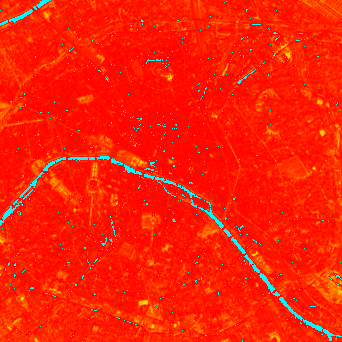
\includegraphics[scale=0.45]{../3_ndvi/images/Paris/12_ndvi.png}
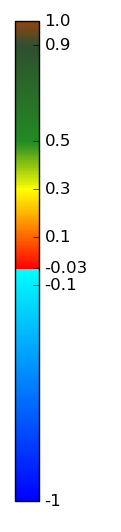
\includegraphics[scale=0.4]{../3_ndvi/images/colormap.png}
}
\begin{center}
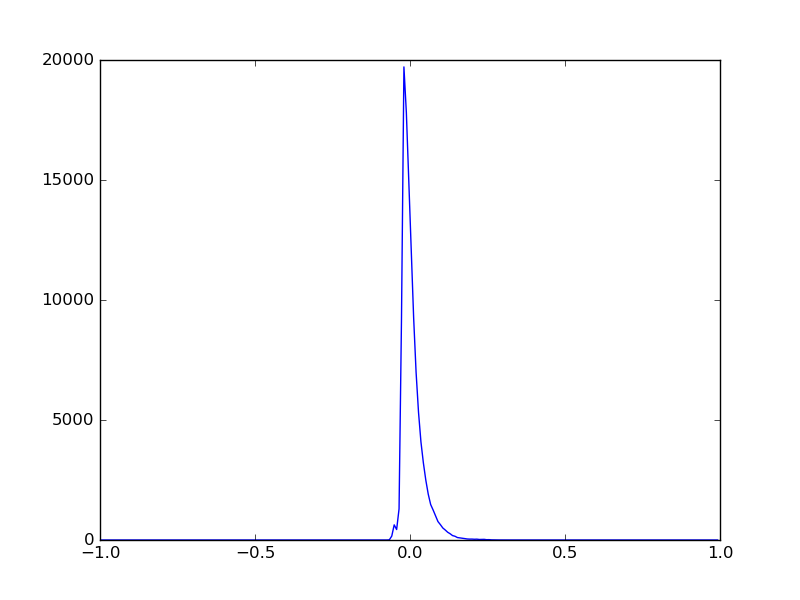
\includegraphics[scale=0.4]{../3_ndvi/images/Paris/12_ndvi_histo.png}
\end{center}
\caption{Image couleur, image $NDVI$ et histogramme de $NDVI$ pour la ville de $Paris$ sur un périmètre de $105$km\textsuperscript{2} au mois de $Decembre$}
\label{paris_ndvi}
\end{figure}

La figure \ref{paris_ndvi} montre un $NDVI$ quasi nulle donc sans végétation, comme on peut s'y attendre dans une commune urbaine telle que Paris en période hivernale.\\

\section{Evolution du NDVI en fonction de la densité de population}

La figure \ref{ndvi_categorie} montre la superposition des courbes de $NDVI$ au mois de $Juillet$ pour plusieurs communes françaises :\\
\begin{figure}[H]
\centerline{
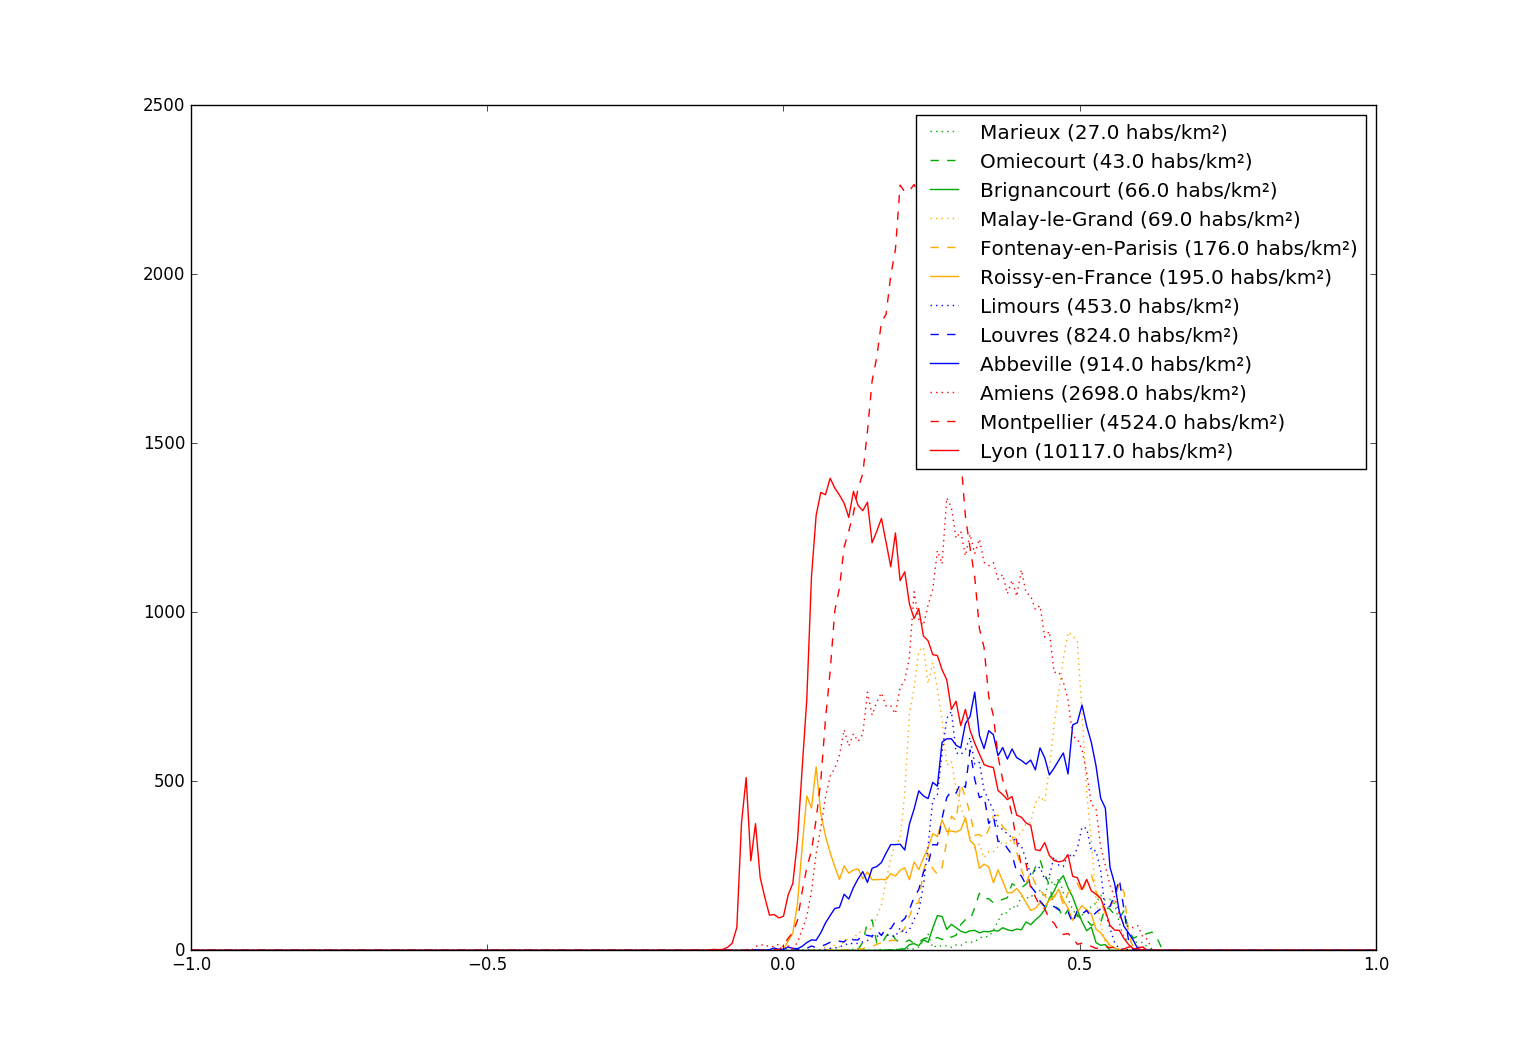
\includegraphics[scale=0.5]{../3_ndvi/images/ndvi_categorie.png}
}
\caption{Superposition des courbes de $NDVI$ pour plusieurs communes françaises métropolitaines}
\label{ndvi_categorie}
\end{figure}
\clearpage

Nous observons donc que les communes les plus denses sont caractérisés par un spectre d'amplitude fort et distribué vers les basses fréquences. A mesure 
qu'on se déplace vers les communes les moins denses, on constate une diminution d'amplitude et un déplacement de la distribution de $NDVI$ vers les
hautes fréquences.\\
Les figures \ref{ndvi_cat1},\ref{ndvi_cat2},\ref{ndvi_cat3} et \ref{ndvi_cat4} présentent les images de $NDVI$ pour ces commues.\\ 

\begin{figure}[H]
\centerline{
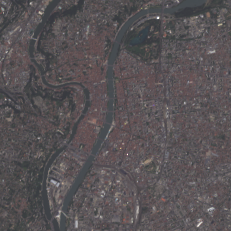
\includegraphics[scale=0.6]{../3_ndvi/images/Lyon/07_rgb.png}
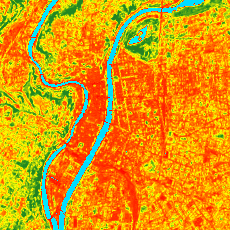
\includegraphics[scale=0.6]{../3_ndvi/images/Lyon/07_ndvi.png}
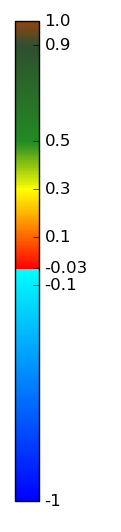
\includegraphics[scale=0.3]{../3_ndvi/images/colormap.png}
}
\centerline{
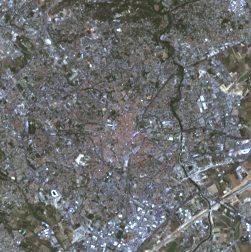
\includegraphics[scale=0.6]{../3_ndvi/images/Montpellier/07_rgb.png}
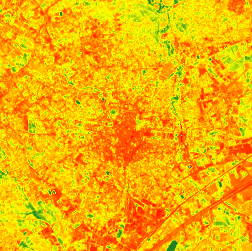
\includegraphics[scale=0.6]{../3_ndvi/images/Montpellier/07_ndvi.png}
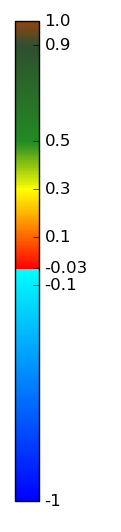
\includegraphics[scale=0.3]{../3_ndvi/images/colormap.png}
}
\centerline{
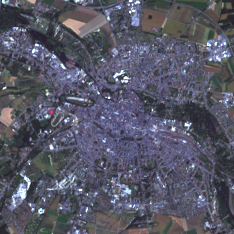
\includegraphics[scale=0.6]{../3_ndvi/images/Amiens/07_rgb.png}
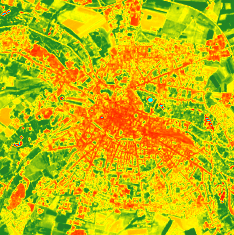
\includegraphics[scale=0.6]{../3_ndvi/images/Amiens/07_ndvi.png}
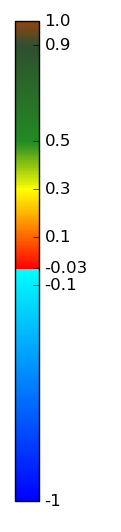
\includegraphics[scale=0.3]{../3_ndvi/images/colormap.png}
}
\caption{Image $NDVI$ et image couleur au mois de $Juillet$ pour les trois communes densément peuplées, de haut en bas respectivement :
$Lyon$ ($10117$ habs/km\textsuperscript{2}),
$Montpellier$ ($4524$ habs/km\textsuperscript{2}),
$Amiens$ ($2689$ habs/km\textsuperscript{2}),
}
\label{ndvi_cat1}
\end{figure}
\clearpage

\begin{figure}[H]
\centerline{
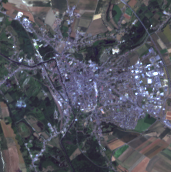
\includegraphics[scale=0.9]{../3_ndvi/images/Abbeville/07_rgb.png}
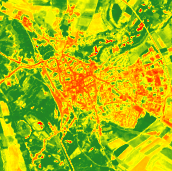
\includegraphics[scale=0.9]{../3_ndvi/images/Abbeville/07_ndvi.png}
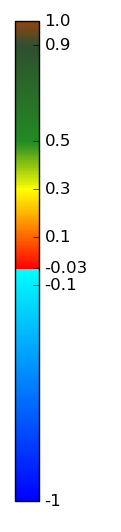
\includegraphics[scale=0.3]{../3_ndvi/images/colormap.png}
}
\centerline{
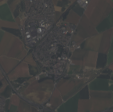
\includegraphics[scale=0.9]{../3_ndvi/images/Louvres/07_rgb.png}
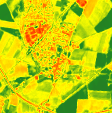
\includegraphics[scale=0.9]{../3_ndvi/images/Louvres/07_ndvi.png}
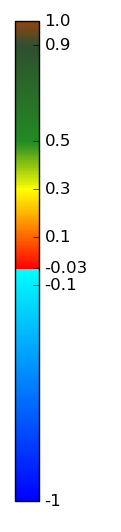
\includegraphics[scale=0.3]{../3_ndvi/images/colormap.png}
}
\centerline{
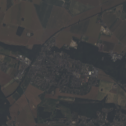
\includegraphics[scale=0.9]{../3_ndvi/images/Limours/07_rgb.png}
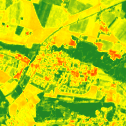
\includegraphics[scale=0.9]{../3_ndvi/images/Limours/07_ndvi.png}
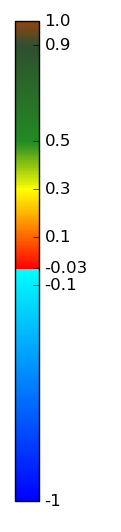
\includegraphics[scale=0.3]{../3_ndvi/images/colormap.png}
}
\caption{Image $NDVI$ et image couleur au mois de $Juillet$ pour les trois communes de densité intermédiaire, de haut en bas respectivement :
$Abbeville$ ($914$ habs/km\textsuperscript{2}),
$Louvres$ ($824$ habs/km\textsuperscript{2}),
$Limours$ ($453$ habs/km\textsuperscript{2}),
}
\label{ndvi_cat2}
\end{figure}
\clearpage

\begin{figure}[H]
\centerline{
\includegraphics[scale=1.1]{../3_ndvi/images/Roissy-en-France/07_rgb.png}
\includegraphics[scale=1.1]{../3_ndvi/images/Roissy-en-France/07_ndvi.png}
\includegraphics[scale=0.3]{../3_ndvi/images/colormap.png}
}
\centerline{
\includegraphics[scale=1.1]{../3_ndvi/images/Fontenay-en-Parisis/07_rgb.png}
\includegraphics[scale=1.1]{../3_ndvi/images/Fontenay-en-Parisis/07_ndvi.png}
\includegraphics[scale=0.3]{../3_ndvi/images/colormap.png}
}
\centerline{
\includegraphics[scale=1.1]{../3_ndvi/images/Malay-le-Grand/07_rgb.png}
\includegraphics[scale=1.1]{../3_ndvi/images/Malay-le-Grand/07_ndvi.png}
\includegraphics[scale=0.3]{../3_ndvi/images/colormap.png}
}
\caption{Image $NDVI$ et image couleur au mois de $Juillet$ pour les trois communes peu denses, de haut en bas respectivement :
$Roissy-en-France$ ($195$ habs/km\textsuperscript{2}),
$Fontenay-en-Parisis$ ($176$ habs/km\textsuperscript{2}),
$Malay-le-Grand$ ($63$ habs/km\textsuperscript{2}),
}
\label{ndvi_cat3}
\end{figure}
\clearpage

\begin{figure}[H]
\centerline{
\includegraphics[scale=1.5]{../3_ndvi/images/Brignancourt/07_rgb.png}
\includegraphics[scale=1.5]{../3_ndvi/images/Brignancourt/07_ndvi.png}
\includegraphics[scale=0.3]{../3_ndvi/images/colormap.png}
}
\centerline{
\includegraphics[scale=1.5]{../3_ndvi/images/Omiecourt/07_rgb.png}
\includegraphics[scale=1.5]{../3_ndvi/images/Omiecourt/07_ndvi.png}
\includegraphics[scale=0.3]{../3_ndvi/images/colormap.png}
}
\centerline{
\includegraphics[scale=1.5]{../3_ndvi/images/Marieux/07_rgb.png}
\includegraphics[scale=1.5]{../3_ndvi/images/Marieux/07_ndvi.png}
\includegraphics[scale=0.3]{../3_ndvi/images/colormap.png}
}
\caption{Image $NDVI$ et image couleur au mois de $Juillet$ pour les trois communes peu denses, de haut en bas respectivement :
$Brignancourt$ ($66$ habs/km\textsuperscript{2}),
$Omiecourt$ ($43$ habs/km\textsuperscript{2}),
$Marieux$ ($27$ habs/km\textsuperscript{2}),
}
\label{ndvi_cat4}
\end{figure}

Utiliser le NDVI à des fins de prédiction de densité présente donc un sens.

\section{Données pour le Machine Learning}

Nous avons à notre disposition un tableau de $34190$ comunes françaises métropolitaines contenant entre autres caractéristiques, les latitude et longitude en degrés,
la surface em km\textsuperscript{2}. Ces informations vont nous permettrent d'extraire les variables explicatives de notre problème.\\
La méthode d'extraction d'information du NDVI pour chaque commune se fait comme suit :
\begin{description}
\item[-] Pour une commune donnée, on projete ses latitude et longitude en Web Mercator. Les positions $x$,$y$ obtenues permettent d'aller récupérer 
la scéne \begin{itshape}Landsat-8\end{itshape} dont le centre est le plus proche de la commune. Prendre la scène la plus proche de cette manière,
permet d'éviter que la commune échoue sur un bord non couvert par une scène.
\item[-] Puis, on découpe un carré de centre les coordonnées de la  commune, et d'aire égale à la surface de la commune.
\item[-] On crée alors l'image de \begin{itshape}NDVI\end{itshape} correspondante
\item[-] On calcule l'histogramme de l'image de \begin{itshape}NDVI\end{itshape} en prenant 1024 bins uniformément répartis dans l'intervalle [-1 1].
\item[-] On obtient ainsi un vecteur descripteur pour la commune
\item[-] On réitère le procédé pour chacune des communes
\end{description}

Nous présentons le procédé à travers l'exemple ci-après \ref{ndvi_extraction} :
\begin{figure}[H]
\centerline{
\includegraphics[scale=0.45]{images/05_rgb.png}
\includegraphics[scale=0.45]{images/05_ndvi.png}
\includegraphics[scale=0.4]{images/colormap.png}
}
\begin{center}
\includegraphics[scale=0.45]{images/05_ndvi_histo.png}
\end{center}
\caption{Image couleur, image $NDVI$ et histogramme de $NDVI$ pour la commune de $Carcassonne$ sur un périmètre de $65.08$km\textsuperscript{2} au mois de $Mai$ 2013}
\label{ndvi_extraction}
\end{figure}

Au final, nos données se présente sous la forme d'un tableau contenant à chaque ligne, l'histogramme d'une commune et sa densité (catégorie). Avec un total
de $34190$ communes métropolitaines.\ref{data_class}.

\begin{table}[H]
\begin{center}
\begin{adjustbox}{max width=\textwidth}
\begin{tabular}{|c|c|c|c|c|c|c|c|c|>{\bfseries}c|}
\hline 
nom &  bin-1 & bin-2 & ... & bin-511 & bin-512 &... & bin-1023 & bin-1024 & densité (catégorie) \\
\hline 
Ozan & 0 & 0 & ... & 1 & 5 & ... & 0 & 0 & 1\\
\hline 
Cormoranche-sur-saone & 0 & 0 & ... & 1 & 4 & ... & 0 & 0 & 1\\
\hline 
Paris & 0 & 0 & ... & 1953 & 1815 & ... & 0 & 0 & 6\\
\hline
Lyon & 0 & 0 & ... & 1099 & 1032 & ... & 0 & 0 & 5\\
\hline
Tours & 0 & 0 & ... & 268 & 238 & ... & 0 & 0 & 3\\
\hline
Besancon & 0 & 0 & ... & 97 & 122 & ... & 0 & 0 & 1\\
\hline 
... & ... & ... & ... & ... & ... & ... & ... & ... & ... \\
\hline
\end{tabular}
\end{adjustbox}
\end{center}
\caption{Variables explicatives (histogramme de $NDVI$) et variable à prédire (densité) par classification, sous forme de tableau}
\label{data_class}
\end{table}

Nous obtenons ainsi des données prêtes pour l'apprentissage automatique.


\chapter{Classification pour la prédiction de densité de population en fonction du NDVI}
 
\section{Score de précision d'un modèle de classification}

Afin de juger de la performance d'un classifieur, on utilisera le score de précision dont la formule est décrite ci-après:\\

\begin{equation}
precision = \frac{\sum \limits_{\underset{}{i=1}}^{n_{validation}} (y_i = p_i)}{n_{validation}}
\end{equation}

avec:
\begin{description}
\item[-] ${y_i}$, l'ensemble des valeurs de densité (catégorie) à prédire pour les échantillons .
\item[-] ${p_i}$, l'ensemble des prédictions associées et calculées via le modèle entrainé.
\end{description}

\section{Cross validation}

Le principe consiste à découper à plusieurs resprises (typiquement 3) et de manière aléatoire, l'ensemble des échantillons en :
\begin{description}
\item[-] une partie (70\% par exemple) dite d'entraînement, servant à entrainer le modèle.
\item[-] une autre partie contenant le reste, dite de validation servant à calculer l'erreur (score de validation) que commet le modèle entrainé obtenu précédemment.
\end{description}
Ainsi, à plusieurs reprises, on obtient un score de validation avec des données aléatoirement selectionnées.
La moyenne de ces scores de validation donne une estimation de la capacité de prédiction du classifieur, leur variance renseigne sur la sensibilité du classifieur au fluctuation des données.\\
Par la suite, nous proposons l'utilisation de trois classifieurs dont nous donnerons les performances en cross-validation :
\begin{description}
\item[-] \begin{itshape}K-plus-proches-voisins\end{itshape}
\item[-] \begin{itshape}Support-Vector-Machine\end{itshape}
\item[-] \begin{itshape}Réseaux de Neurones\end{itshape}
\end{description}


\section{Métriques pour l'analyse des résultats}

Afin d'aller plus en détails dans l'etude des classifieurs, on montrera pour chacun d'eux :
\begin{description}
 \item [-] La matrice de confusion qui premet d'observer le comportement des erreurs d'une classe donnée
 \item[-] Les courbes ROC (Receiver Operating Characteristic) permettent de visualiser pour chaque classe, la probabilité de détection en fonction de la probabilité de fausse alarme (cela n'est possible que si le classifieur peut
 fournir des probabilités d'appartenance à chaque classe lors de la prédiction, ce qui est le cas des classifieurs utilisés ici).
 \item[-] l'AUC (Area Under Curve) est pour chaque classe, l'aire sous sa courbe ROC. Une valeur proche de 1 signifie une bonne performance en détection et en fausse alarme pour la classe donnée.
\end{description}
 

\section{Disproportion des classes}
Ainsi que nous le présentons dans le tableau \ref{imbalanced}, il existe une forte disproportion entre les six différentes classes (un facteur de 2000 entre la catégorie 1 et la catégorie 5). 
Cela devra être pris en compte afin de ne pas obtenir un classifieur constant prédisant la classe majoritaire.

\begin{table}[H]
\begin{center}
\begin{adjustbox}{max width=\textwidth}
{
\begin{tabular}{|c|c|}
   \hline
  catégorie & nombre d'échantillons\\
  \hline
  \textbf{1} & 32533\\
  \hline
  \textbf{2} & 1252\\
  \hline
  \textbf{3} & 288\\
  \hline
  \textbf{4} & 78\\
  \hline
  \textbf{5} & 15\\
  \hline
  \textbf{6} & 24 \\
  \hline
\end{tabular}
}
\end{adjustbox}
\end{center}
\caption{Nombre d'échantillons par classe pour les données de communes françaises}
\label{imbalanced}
\end{table}

\section{K Plus Proches Voisins}

\subsection{Suréchantillonage par synthétisation}
Afin de surmonter la problème lié à la disproportion de classes, on va procéder à un suréchantillonnage des données minoritaires par synthéstisation. Le principe, connu sous le nom SMOTE \cite{smote} (pour 
Synthetic Minority Oversampling TEchnique), consiste à créer une nouvelle donnée de la classe minoritaire sur la droite joignant deux points de cette classe, en choisissant celui qui maximise la distance aux autres classes.\\
La figure \ref{smote} donne un aperçu graphique du procédé.

\begin{figure}[H]
 \begin{center}
 \includegraphics[scale=0.3]{../5_diaporama/images/oversampling/smote.png}
 \caption{Illustration de la technique SMOTE de suréchantillonage d'une classe minoritaire $i$}
 \label{smote}
 \end{center}
\end{figure}

On réitère ainsi le procédé pour plusieurs couples de points de la classe minoritaire jusqu'à atteindre un nombre de points
égale à ceux de la classe majoritaire.\\
Cette densification donne plus d'influence aux données de la classe minoritaire lors de l'attribution des $k$ voisins.\\

\subsection{Résultats}

Nous obtenons un score moyen de 94.74\% en cross-validation pour un nombre de voisins $k$ égal à $5$. \\
Après ré-entrainement du classifieur avec $k$=5, sur tous les échantillons, on obtient les matrices de confusion \ref{knn_cm} et courbes ROC \ref{knn_roc} suivantes :

\begin{table}[H]
  \begin{center}
  \begin{adjustbox}{max width=\textwidth}
  \begin{tabular}{|c|c|c|c|c|c|c|}
    \hline
    \multicolumn{7}{|c|}{{ \begin{bf}Confusion matrix after refitting\end{bf}}} \\
    \hline
     & \textbf{1} & \textbf{2} & \textbf{3} & \textbf{4} & \textbf{5} & \textbf{6}\\
    \hline
    \textbf{1} & 32533 & 0 & 0 & 0 & 0 & 0\\
    \hline
    \textbf{2} & 0 & 1252 & 0 & 0 & 0 & 0\\
    \hline
    \textbf{3} & 0 & 0 & 288 & 0 & 0 & 0\\
    \hline
    \textbf{4} & 0 & 0 & 0 & 78 & 0 & 0\\
    \hline
    \textbf{5} & 0 & 0 & 0 & 0 & 15 & 0\\
    \hline
    \textbf{6} & 0 & 0 & 0 & 0 & 0 & 24\\
    \hline
  \end{tabular}
  \end{adjustbox}
  \end{center}
  \caption{Matrice de confusion pour le classifieur de K-plus-proches-voisins - France}
  \label{knn_cm}
\end{table}

\begin{figure}[H]
 \begin{center}
\includegraphics[scale=0.4]{../../data/France/test/Nearest_Neighboors_Classification/Nearest_Neighboors_Classification_roc.png}
 \end{center}
 \caption{Courbes ROC pour le classifieur de K-plus-proches-voisins - France}
 \label{knn_roc}
\end{figure}

On note une prediction parfaite (score de 100\%) lorsque le modèle est entrainé sur toutes les données. Cela alors qu'on avait un score de 94.74\% lors du découpage en entrainement/vaildation. Cela dénote une forte fluctuation 
du score en fonction des données utilisées et donc une variance trop grande du classifieur (sur-apprentissage).

\section{Support Vector Machine à noyau gaussien}

\subsection{Régularisation}

Ce classifieur cherche pour chaque classe, l'hyperplan qui la sépare des autres avec les marges les plus vastes possibles (on parle d'hyperplan optimal). Au préalable, on projète les données dans un espace de plus grande 
dimension, potentiellement infini (c'est la cas du noyau gaussien) où les données pourront être eventuellement linéairement séparables.\\
Afin de forcer la bonne classification des classes minoritaires, il convient de donner de l'importance à celles-ci en pénalisant leurs mauvaises classifications. On le fait en attribuant un fort paramètre de régularisation 
aux classes manioritaires lors de la recherche opérationelle de leur hyperplan optimal respectif.\\
Ainsi, on prendra un paramètre de régularisation $C_{i}$ pour la classe $i$ inversement proportionnel au nombre d'échantillons $n_{i}$ de la classe $i$ : $C_{i} = \frac{n}{n_i}$.\\
On montre à quel point un fort paramètre de régularisation $C$ est crucial pour bien classer
une classe minoritaire à travers l'exemple suivant créé via le site de la librairie \begin{itshape}LIBSVM\end{itshape}\cite{libsvm}.\\


\begin{figure}[H]
 \begin{center}
\includegraphics[scale=0.5]{images/svm/svm_g_001_100.png}
\includegraphics[scale=0.5]{images/svm/svm_g_001_1000.png}
 \caption{SVM à noyau gaussien ($\gamma=100$) avec $C=100$ (mauvaise classification) et avec $C=1000$ (bonne classification)}
 \label{svm_exemple}
 \end{center}
\end{figure}
\subsection{Résultats}

Nous obtenons un score moyen de 84.04\% en cross-validation pour un coefficient de noyau gaussien $\gamma = 0.01$. \\
Après ré-entrainement du classifieur sur tous les échantillons, on obtient les matrices de confusion \ref{svm_cm} et courbes ROC \ref{svm_roc} suivantes :

\begin{table}[H]
  \begin{center}
\begin{adjustbox}{max width=\textwidth}
  \begin{tabular}{|c|c|c|c|c|c|c|}
    \hline
    \multicolumn{7}{|c|}{{ \begin{bf}Confusion matrix after refitting\end{bf}}} \\
    \hline
     & \textbf{1} & \textbf{2} & \textbf{3} & \textbf{4} & \textbf{5} & \textbf{6}\\
    \hline
    \textbf{1} & 28569 & 3632 & 251 & 51 & 27 & 3\\
    \hline
    \textbf{2} & 77 & 1021 & 139 & 11 & 1 & 3\\
    \hline
    \textbf{3} & 1 & 25 & 254 & 7 & 0 & 1\\
    \hline
    \textbf{4} & 0 & 0 & 3 & 75 & 0 & 0\\
    \hline
    \textbf{5} & 0 & 0 & 0 & 0 & 15 & 0\\
    \hline
    \textbf{6} & 0 & 0 & 0 & 0 & 0 & 24\\
    \hline
  \end{tabular}
  \end{adjustbox}
  \caption{Matrice de confusion pour le classifieur SVM gaussien - France}
  \label{svm_cm}
  \end{center}
\end{table}

\begin{figure}[H]
 \begin{center}
\includegraphics[scale=0.4]{../../data/France/test/Support_Vector_Gaussian_Classification/Support_Vector_Gaussian_Classification_roc.png}
 \caption{Courbes ROC pour le classifieur SVM - France}
 \label{svm_roc}
 \end{center}
\end{figure}

On note cette fois-ci l'absence de surapprentissage. En effet, la valeur $\gamma=0.01$ utilisée évite la formation de frontière trop complexe, comme nous le montrons dans l'exemple simple
suivant \ref{svm_exemple2}.\\
\begin{figure}[H]
 \begin{center}
\includegraphics[scale=0.5]{images/svm/svm_g_100.png}
\includegraphics[scale=0.5]{images/svm/svm_g_001.png}
 \caption{SVM à noyau gaussien avec $\gamma=100$ (sur-apprentissage) et avec $\gamma=0.01$ (pas de sur-apprentissage)}
 \label{svm_exemple2}
 \end{center}
\end{figure}

Enfin, on peut aussi comparer la prédiction à la vérité terrain en affichant nos échantillons sur une carte \ref{svm_carte}.

\begin{figure}[H]
\centerline{
\includegraphics[scale=0.5]{../../data/France/test/Support_Vector_Gaussian_Classification/Support_Vector_Gaussian_Classification/density_ground_truth.png}
\includegraphics[scale=0.5]{../../data/France/test/Support_Vector_Gaussian_Classification/Support_Vector_Gaussian_Classification/density_classification.png}
}
\caption{Carte verité-terrain (à gauche) et prédiction (à droite) pour le classifieur SVM - France}
\label{svm_carte}
\end{figure}

\section{Réseau de Neurones}

\subsection{Pondération des erreurs de classification}

Un réseau de neurones corrige ses coefficients par rétro-propagation des erreurs qu'il commet, cela de manière itérative sur les données. Afin de tenir compte de la rareté des échantillons de classe minoritaire, 
il convient de pondérer les erreurs . Ainsi, on donnera plus de poids aux erreurs liées à la classe minoritaire en attribuant le facteur multiplicatif $w_i=\frac{n_1}{n_i}$ à la classe $i$.\\

\subsection{Résultats}

Nous obtenons un score moyen de 90.46\% en cross-validation pour une couche à $1200$ neurones. \\
Après ré-entrainement du classifieur sur tous les échantillons, on obtient les matrices de confusion \ref{nn_cm} et courbes ROC \ref{nn_roc} suivantes :

\begin{table}[H]
  \begin{center}
\begin{adjustbox}{max width=\textwidth}
  \begin{tabular}{|c|c|c|c|c|c|c|}
    \hline
    \multicolumn{7}{|c|}{{ \begin{bf}Confusion matrix after refitting\end{bf}}} \\
    \hline
     & \textbf{1} & \textbf{2} & \textbf{3} & \textbf{4} & \textbf{5} & \textbf{6}\\
    \hline
    \textbf{1} & 29743 & 2281 & 367 & 95 & 24 & 23\\
    \hline
    \textbf{2} & 207 & 853 & 164 & 23 & 2 & 3\\
    \hline
    \textbf{3} & 2 & 36 & 236 & 9 & 2 & 3\\
    \hline
    \textbf{4} & 0 & 0 & 2 & 76 & 0 & 0\\
    \hline
    \textbf{5} & 0 & 0 & 0 & 0 & 15 & 0\\
    \hline
    \textbf{6} & 0 & 0 & 0 & 0 & 0 & 24\\
    \hline
  \end{tabular}
  \end{adjustbox}
  \caption{Matrice de confusion pour le classifieur Réseaux de Neurones - France}
  \label{nn_cm}
  \end{center}
\end{table}

\begin{figure}[H]
 \begin{center}
\includegraphics[scale=0.4]{../../data/France/test/Neural_Network_Classification-oversampling/Neural_Network_Classification-oversampling_roc.png}
 \caption{Courbes ROC pour le classifieur Réseaux de Neurones - France}
 \label{nn_roc}
 \end{center}
\end{figure}


\begin{figure}[H]
\centerline{
\includegraphics[scale=0.5]{../../data/France/test/Neural_Network_Classification-oversampling/Neural_Network_Classification-oversampling/density_ground_truth.png}
\includegraphics[scale=0.5]{../../data/France/test/Neural_Network_Classification-oversampling/Neural_Network_Classification-oversampling/density_classification.png}
}
\caption{Carte verité-terrain (à gauche) et prédiction (à droite) pour le classifieur Réseaux de Neurones - France}
\label{nn_carte}
\end{figure}

On note là encore que le surapprentissage est évité. Cela car on a activé l'option dite de \og early stopping \fg{}. En effet, lorsque l'entrainement d'un algorithme se fait de manière itératif, il convient
de calculer le score de validation à chaque itération (ou epoch) et stopper l'entrainement dès lors que le score de validation n'augmente plus. Sinon, on laisse le classifieur se spécifier sur les données d'entrainement
au détriment d'une meilleure généralisation sur les données de validation.
La figure \ref{early} illustre le procédé.

\begin{figure}[H]
\centerline{
\includegraphics[scale=0.5]{images/earlystopping.png}
}
\caption{Illustration de l'option de \og early stopping \fg{} pour un algorithme à entrainement itératif}
\label{early}
\end{figure}


\section{Influence nuageuse}

Les résultats du Réseaux de Neurones montre que la couverture nuageuse a une certaine influence sur la prédiction.
En effet, on remarque que la region corse, les côtes d'Armor et le Nord-Pas-de-Calais se voient prédire une densité très élevé (catégorie 5/6). Lorsqu'on 
affiche d'un côté la couverture nuageuse de chaque échantillon (via l'image de qualité fournit par \begin{itshape}Landsat-8\end{itshape}) et 
l'erreur de prédiction, on constate une certaine corrélation \ref{nuage}.

\begin{figure}[H]
\centerline{
\includegraphics[scale=0.5]{../../data/France/test/Neural_Network_Classification-oversampling/Neural_Network_Classification-oversampling/density_covering.png}
\includegraphics[scale=0.5]{../../data/France/test/Neural_Network_Classification-oversampling/Neural_Network_Classification-oversampling/density_classification_error.png}
}
\caption{Couverture nuageuse en \% à gauche, erreur de classification $y_{pred}-y_{true}$  à droite}
\label{nuage}
\end{figure}

Illustrons le phénomène plus en détail, à travers les communes de \begin{itshape}Silvareccio\end{itshape} et \begin{itshape}Porri\end{itshape}.\\
La première comporte une couverture nuageuse de 49.5\%, de 0\% pour la seconde.\\
Par ailleurs, la première se voit prédire une densité de catégorie 6 au lieu de 1, la seconde se voir correctement prédire la catégorie 1.\\
Les figures \ref{Silvareccio} et \ref{Porri} présentent l'image couleur, l'image NDVI et l'histogramme de NDVI pour ces deux communes.

\begin{figure}[H]
\begin{center}
    \includegraphics[scale=1.80]{../5_diaporama/images/Silvareccio/08_rgb.png}
    \includegraphics[scale=1.80]{../5_diaporama/images/Silvareccio/08_ndvi.png}
    \includegraphics[scale=0.21]{../5_diaporama/images/Silvareccio/08_ndvi_histo.png}
\end{center}
\caption{Image couleur, image de NDVI et histogramme de NDVI - Silvareccio, Corse - couverture nuageuse de 49.5\%}
\label{Silvareccio}
\end{figure}
 
\begin{figure}[H]
\begin{center}
    \includegraphics[scale=1.80]{../5_diaporama/images/Porri/08_rgb.png}
    \includegraphics[scale=1.80]{../5_diaporama/images/Porri/08_ndvi.png}
    \includegraphics[scale=0.21]{../5_diaporama/images/Porri/08_ndvi_histo.png}
\end{center}
\caption{Image couleur, image de NDVI et histogramme de NDVI - Porri, Corse - couverture nuageuse de 0\%}
\label{Porri}
\end{figure} 

On constate que la couverture nuageuse renvoit un NDVI à valeurs proches de 0, soit le NDVI d'un sol nu qui caractérise les villes très denses. Cela peut expliquer la surévaluation de la densité dans un grand nombre
de petites communes nuageuses.
 
\chapter{Test pour la prédiction de densité de population en fonction du NDVI}

\section{Données de test}

Nous avons pu récupérer les métadonnées nécessaires à la labélisation et l'extraction des features pour les communes de trois pays limitrophes de la France : Suisse \cite{suisse}, Belgique \cite{belgique}, Pays-Bas\cite{pays-bas}.\\
Les tableaux \ref{suisse_data}, \ref{belgique_data} et \ref{pays-bas_data} montrent la distribution des catégories associées.

   \begin{table}[H]
   \begin{center}
   \begin{adjustbox}{max width=0.5\textwidth}
    \begin{tabular}{|c|c|}
      \hline
      \multicolumn{2}{|c|}{\begin{bf}Suisse (2013)\end{bf}} \\
      \hline
      \textbf{categorie} & \textbf{nombre d'échantillons}\\
      \hline
      \textbf{1} & 1857\\
      \hline
      \textbf{2} & 428\\
      \hline
      \textbf{3} & 57\\
      \hline
      \textbf{4} & 9\\
      \hline
      \textbf{5} & 1\\
      \hline
      \textbf{6} & 0 \\
      \hline
      \textbf{total} & 2352\\
      \hline
    \end{tabular}
   \end{adjustbox}
   \caption{Données des densités pour la Suisse (recensement 2013)}
   \label{suisse_data}
   \end{center}
   \end{table}

   \begin{table}[H]
   \begin{center}
   \begin{adjustbox}{max width=0.5\textwidth}
    \begin{tabular}{|c|c|}
      \hline
      \multicolumn{2}{|c|}{\begin{bf}Belgique (2015)\end{bf}} \\
      \hline
      \textbf{categorie} & \textbf{nombre d'échantillons}\\
      \hline
      \textbf{1} & 406\\
      \hline
      \textbf{2} & 154\\
      \hline
      \textbf{3} & 14\\
      \hline
      \textbf{4} & 7\\
      \hline
      \textbf{5} & 1\\
      \hline
      \textbf{6} & 7\\
      \hline
      \textbf{total} & 589\\
      \hline
    \end{tabular}
   \end{adjustbox}
   \caption{Données des densités pour la Belgique (recensement 2015)}
   \label{belgique_data}
   \end{center}
   \end{table}

   \begin{table}[H]
   \begin{center}
   \begin{adjustbox}{max width=0.5\textwidth}
    \begin{tabular}{|c|c|}
      \hline
      \multicolumn{2}{|c|}{\begin{bf}Pays-Bas (2014)\end{bf}} \\
      \hline
      \textbf{categorie} & \textbf{nombre d'échantillons}\\
      \hline
      \textbf{1} & 234\\
      \hline
      \textbf{2} & 121\\
      \hline
      \textbf{3} & 31\\
      \hline
      \textbf{4} & 1\\
      \hline
      \textbf{5} & 0\\
      \hline
      \textbf{6} & 0 \\
      \hline
      \textbf{total} & 388\\
      \hline
    \end{tabular}
   \end{adjustbox}
   \caption{Données des densités pour les Pays-Bas (recensement 2014)}
   \label{pays-bas_data}
   \end{center}
   \end{table}
   
   
 Par ailleurs, nous avons récupére les données \begin{itshape}Landsat-8\end{itshape} pour ces trois pays, à chaque fois pour l'année correspondante, entre Mai et Septembre, avec une couverture
 nuageuse inférieur à 20\%. Nous montrons ci-après la projection \begin{itshape}Web Mercator\end{itshape} des images récupérées.
 
 \begin{figure}[H]
 \begin{center}
 \includegraphics[scale=0.60]{../../data/Suisse/covering-selection.png}
 \caption{Projection Web Mercator des images Landsat-8 pour la Suisse - Mai à Septembre 2013}
\label{suisse_landsat}
\end{center}
\end{figure}

 \begin{figure}[H]
 \begin{center}
 \includegraphics[scale=0.60]{../../data/Belgique/covering-selection.png}
 \caption{Projection Web Mercator des images Landsat-8 pour la Belgique - Mai à Septembre 2015}
\label{belgique_landsat}
\end{center}
\end{figure}

 \begin{figure}[H]
 \begin{center}
 \includegraphics[scale=0.60]{../../data/Pays-Bas/covering-selection.png}
 \caption{Projection Web Mercator des images Landsat-8 pour les Pays-Bas - Mai à Septembre 2014}
\label{pays-bas_landsat}
\end{center}
\end{figure}

Dans ce qui suit, nous avons l'opportunité de tester la généralisation de nos trois classifieurs.\\
Pour chacun d'eux, nous présenterons les mêmes métriques (matrice de confusion, courbes ROC et AUC) en testant les commues suisses, belges et néerlandaises respectivement.

\section{K Plus Proches Voisins}

\subsection{Suisse}

\begin{table}[H]
  \begin{center}
  \begin{adjustbox}{max width=\textwidth}
  \begin{tabular}{|c|c|c|c|c|c|c|}
    \hline
    \multicolumn{7}{|c|}{{ \begin{bf}Confusion matrix after refitting\end{bf}}} \\
    \hline
     & \textbf{1} & \textbf{2} & \textbf{3} & \textbf{4} & \textbf{5} & \textbf{6}\\
    \hline
    \textbf{1} & 1411 & 396 & 33 & 8 & 3 & 6\\
    \hline
    \textbf{2} & 114 & 268 & 40 & 6 & 0 & 0\\
    \hline
    \textbf{3} & 1 & 35 & 16 & 5 & 0 & 0\\
    \hline
    \textbf{4} & 1 & 4 & 2 & 0 & 1 & 1\\
    \hline
    \textbf{5} & 0 & 0 & 0 & 0 & 1 & 0\\
    \hline
    \textbf{6} & 0 & 0 & 0 & 0 & 0 & 0\\
    \hline
  \end{tabular}
  \end{adjustbox}
  \end{center}
  \caption{Matrice de confusion pour le classifieur de K-plus-proches-voisins - Suisse}
  \label{knn_cm_suisse}
\end{table}

\begin{figure}[H]
 \begin{center}
\includegraphics[scale=0.4]{../../data/Suisse/test/Nearest_Neighboors_Classification/Nearest_Neighboors_Classification_roc.png}
 \end{center}
 \caption{Courbes ROC pour le classifieur de K-plus-proches-voisins - Suisse}
 \label{knn_roc_suisse}
\end{figure}

\begin{figure}[H]
\centerline{
\includegraphics[scale=0.5]{../../data/Suisse/test/Nearest_Neighboors_Classification/Nearest_Neighboors_Classification/density_ground_truth.png}
\includegraphics[scale=0.5]{../../data/Suisse/test/Nearest_Neighboors_Classification/Nearest_Neighboors_Classification/density_classification.png}
}
\caption{Carte verité-terrain (à gauche) et prédiction (à droite) pour le classifieur de K-plus-proches-voisins - Suisse}
\label{nn_carte_suisse}
\end{figure}


\subsection{Belgique}

\begin{table}[H]
  \begin{center}
  \begin{adjustbox}{max width=\textwidth}
  \begin{tabular}{|c|c|c|c|c|c|c|}
    \hline
    \multicolumn{7}{|c|}{{ \begin{bf}Confusion matrix after refitting\end{bf}}} \\
    \hline
     & \textbf{1} & \textbf{2} & \textbf{3} & \textbf{4} & \textbf{5} & \textbf{6}\\
    \hline
    \textbf{1} & 351 & 48 & 7 & 0 & 0 & 0\\
    \hline
    \textbf{2} & 59 & 71 & 19 & 4 & 1 & 0\\
    \hline
    \textbf{3} & 1 & 6 & 5 & 2 & 0 & 0\\
    \hline
    \textbf{4} & 0 & 0 & 2 & 3 & 2 & 0\\
    \hline
    \textbf{5} & 0 & 0 & 1 & 0 & 0 & 0\\
    \hline
    \textbf{6} & 0 & 0 & 2 & 3 & 0 & 2\\
    \hline
  \end{tabular}
  \end{adjustbox}
  \end{center}
  \caption{Matrice de confusion pour le classifieur de K-plus-proches-voisins - Belgique}
  \label{knn_cm_belgique}
\end{table}

\begin{figure}[H]
 \begin{center}
\includegraphics[scale=0.4]{../../data/Belgique/test/Nearest_Neighboors_Classification/Nearest_Neighboors_Classification_roc.png}
 \end{center}
 \caption{Courbes ROC pour le classifieur de K-plus-proches-voisins - Belgique}
 \label{knn_roc_belgique}
\end{figure}

\begin{figure}[H]
\centerline{
\includegraphics[scale=0.5]{../../data/Belgique/test/Nearest_Neighboors_Classification/Nearest_Neighboors_Classification/density_ground_truth.png}
\includegraphics[scale=0.5]{../../data/Belgique/test/Nearest_Neighboors_Classification/Nearest_Neighboors_Classification/density_classification.png}
}
\caption{Carte verité-terrain (à gauche) et prédiction (à droite) pour le classifieur de K-plus-proches-voisins - Belgique}
\label{nn_carte_belgique}
\end{figure}

\subsection{Pays-Bas}

\begin{table}[H]
  \begin{center}
  \begin{adjustbox}{max width=\textwidth}
  \begin{tabular}{|c|c|c|c|c|c|c|}
    \hline
    \multicolumn{7}{|c|}{{ \begin{bf}Confusion matrix after refitting\end{bf}}} \\
    \hline
     & \textbf{1} & \textbf{2} & \textbf{3} & \textbf{4} & \textbf{5} & \textbf{6}\\
    \hline
    \textbf{1} & 187 & 38 & 9 & 0 & 0 & 0\\
    \hline
    \textbf{2} & 41 & 46 & 28 & 4 & 0 & 2\\
    \hline
    \textbf{3} & 2 & 6 & 16 & 6 & 1 & 0\\
    \hline
    \textbf{4} & 0 & 0 & 1 & 1 & 0 & 0\\
    \hline
    \textbf{5} & 0 & 0 & 0 & 0 & 0 & 0\\
    \hline
    \textbf{6} & 0 & 0 & 0 & 0 & 0 & 0\\
    \hline
  \end{tabular}
  \end{adjustbox}
  \end{center}
  \caption{Matrice de confusion pour le classifieur de K-plus-proches-voisins - Pays-Bas}
  \label{knn_cm_pays-bas}
\end{table}

\begin{figure}[H]
 \begin{center}
\includegraphics[scale=0.4]{../../data/Pays-Bas/test/Nearest_Neighboors_Classification/Nearest_Neighboors_Classification_roc.png}
 \end{center}
 \caption{Courbes ROC pour le classifieur de K-plus-proches-voisins - Pays-Bas}
 \label{knn_roc_pays-bas}
\end{figure}

\begin{figure}[H]
\centerline{
\includegraphics[scale=0.5]{../../data/Pays-Bas/test/Nearest_Neighboors_Classification/Nearest_Neighboors_Classification/density_ground_truth.png}
\includegraphics[scale=0.5]{../../data/Pays-Bas/test/Nearest_Neighboors_Classification/Nearest_Neighboors_Classification/density_classification.png}
}
\caption{Carte verité-terrain (à gauche) et prédiction (à droite) pour le classifieur de K-plus-proches-voisins - Pays-Bas}
\label{nn_carte_pays-bas}
\end{figure}


\section{Support Vector Machine à noyau gaussien}

\subsection{Suisse}

\begin{table}[H]
  \begin{center}
  \begin{adjustbox}{max width=\textwidth}
  \begin{tabular}{|c|c|c|c|c|c|c|}
    \hline
    \multicolumn{7}{|c|}{{ \begin{bf}Confusion matrix after refitting\end{bf}}} \\
    \hline
     & \textbf{1} & \textbf{2} & \textbf{3} & \textbf{4} & \textbf{5} & \textbf{6}\\
    \hline
    \textbf{1} & 1471 & 381 & 3 & 1 & 1 & 0\\
    \hline
    \textbf{2} & 114 & 296 & 17 & 0 & 1 & 0\\
    \hline
    \textbf{3} & 5 & 37 & 14 & 1 & 0 & 0\\
    \hline
    \textbf{4} & 1 & 0 & 6 & 0 & 1 & 1\\
    \hline
    \textbf{5} & 1 & 0 & 0 & 0 & 0 & 0\\
    \hline
    \textbf{6} & 0 & 0 & 0 & 0 & 0 & 0\\
    \hline
  \end{tabular}
  \end{adjustbox}
  \end{center}
  \caption{Matrice de confusion pour le classifieur de SVM - Suisse}
  \label{svm_cm_suisse}
\end{table}

\begin{figure}[H]
 \begin{center}
\includegraphics[scale=0.4]{../../data/Suisse/test/Support_Vector_Gaussian_Classification/Support_Vector_Gaussian_Classification_roc.png}
 \end{center}
 \caption{Courbes ROC pour le classifieur de SVM - Suisse}
 \label{svm_roc_suisse}
\end{figure}

\begin{figure}[H]
\centerline{
\includegraphics[scale=0.5]{../../data/Suisse/test/Support_Vector_Gaussian_Classification/Support_Vector_Gaussian_Classification/density_ground_truth.png}
\includegraphics[scale=0.5]{../../data/Suisse/test/Support_Vector_Gaussian_Classification/Support_Vector_Gaussian_Classification/density_classification.png}
}
\caption{Carte verité-terrain (à gauche) et prédiction (à droite) pour le classifieur de SVM - Suisse}
\label{svm_carte_suisse}
\end{figure}

\subsection{Belgique}

\begin{table}[H]
  \begin{center}
  \begin{adjustbox}{max width=\textwidth}
  \begin{tabular}{|c|c|c|c|c|c|c|}
    \hline
    \multicolumn{7}{|c|}{{ \begin{bf}Confusion matrix after refitting\end{bf}}} \\
    \hline
     & \textbf{1} & \textbf{2} & \textbf{3} & \textbf{4} & \textbf{5} & \textbf{6}\\
    \hline
    \textbf{1} & 378 & 28 & 0 & 0 & 0 & 0\\
    \hline
    \textbf{2} & 88 & 59 & 6 & 1 & 0 & 0\\
    \hline
    \textbf{3} & 2 & 7 & 3 & 2 & 0 & 0\\
    \hline
    \textbf{4} & 1 & 1 & 3 & 1 & 0 & 1\\
    \hline
    \textbf{5} & 0 & 0 & 1 & 0 & 0 & 0\\
    \hline
    \textbf{6} & 1 & 1 & 0 & 1 & 0 & 4\\
    \hline
  \end{tabular}
  \end{adjustbox}
  \end{center}
  \caption{Matrice de confusion pour le classifieur de SVM - Belgique}
  \label{svm_cm_belgique}
\end{table}

\begin{figure}[H]
 \begin{center}
\includegraphics[scale=0.4]{../../data/Belgique/test/Support_Vector_Gaussian_Classification/Support_Vector_Gaussian_Classification_roc.png}
 \end{center}
 \caption{Courbes ROC pour le classifieur de SVM - Belgique}
 \label{svm_roc_belgique}
\end{figure}

\begin{figure}[H]
\centerline{
\includegraphics[scale=0.5]{../../data/Belgique/test/Support_Vector_Gaussian_Classification/Support_Vector_Gaussian_Classification/density_ground_truth.png}
\includegraphics[scale=0.5]{../../data/Belgique/test/Support_Vector_Gaussian_Classification/Support_Vector_Gaussian_Classification/density_classification.png}
}
\caption{Carte verité-terrain (à gauche) et prédiction (à droite) pour le classifieur de SVM - Belgique}
\label{svm_carte_belgique}
\end{figure}


\subsection{Pays-Bas}

\begin{table}[H]
  \begin{center}
  \begin{adjustbox}{max width=\textwidth}
  \begin{tabular}{|c|c|c|c|c|c|c|}
    \hline
    \multicolumn{7}{|c|}{{ \begin{bf}Confusion matrix after refitting\end{bf}}} \\
    \hline
     & \textbf{1} & \textbf{2} & \textbf{3} & \textbf{4} & \textbf{5} & \textbf{6}\\
    \hline
    \textbf{1} & 233 & 1 & 0 & 0 & 0 & 0\\
    \hline
    \textbf{2} & 80 & 32 & 8 & 1 & 0 & 0\\
    \hline
    \textbf{3} & 12 & 8 & 7 & 4 & 0 & 0\\
    \hline
    \textbf{4} & 2 & 0 & 0 & 0 & 0 & 0\\
    \hline
    \textbf{5} & 0 & 0 & 0 & 0 & 0 & 0\\
    \hline
    \textbf{6} & 0 & 0 & 0 & 0 & 0 & 0\\
    \hline
  \end{tabular}
  \end{adjustbox}
  \end{center}
  \caption{Matrice de confusion pour le classifieur de SVM - Pays-Bas}
  \label{svm_cm_pays-bas}
\end{table}

\begin{figure}[H]
 \begin{center}
\includegraphics[scale=0.4]{../../data/Pays-Bas/test/Support_Vector_Gaussian_Classification/Support_Vector_Gaussian_Classification_roc.png}
 \end{center}
 \caption{Courbes ROC pour le classifieur de SVM - Pays-Bas}
 \label{svm_roc_pays-bas}
\end{figure}

\begin{figure}[H]
\centerline{
\includegraphics[scale=0.5]{../../data/Pays-Bas/test/Support_Vector_Gaussian_Classification/Support_Vector_Gaussian_Classification/density_ground_truth.png}
\includegraphics[scale=0.5]{../../data/Pays-Bas/test/Support_Vector_Gaussian_Classification/Support_Vector_Gaussian_Classification/density_classification.png}
}
\caption{Carte verité-terrain (à gauche) et prédiction (à droite) pour le classifieur de SVM - Pays-Bas}
\label{svm_carte_pays-bas}
\end{figure}


\section{Réseau de Neurones}

\subsection{Suisse}

\begin{table}[H]
  \begin{center}
  \begin{adjustbox}{max width=\textwidth}
  \begin{tabular}{|c|c|c|c|c|c|c|}
    \hline
    \multicolumn{7}{|c|}{{ \begin{bf}Confusion matrix after refitting\end{bf}}} \\
    \hline
     & \textbf{1} & \textbf{2} & \textbf{3} & \textbf{4} & \textbf{5} & \textbf{6}\\
    \hline
    \textbf{1} & 1601 & 244 & 7 & 4 & 1 & 0\\
    \hline
    \textbf{2} & 158 & 249 & 18 & 2 & 1 & 0\\
    \hline
    \textbf{3} & 2 & 36 & 16 & 3 & 0 & 0\\
    \hline
    \textbf{4} & 1 & 0 & 5 & 1 & 0 & 2\\
    \hline
    \textbf{5} & 1 & 0 & 0 & 0 & 0 & 0\\
    \hline
    \textbf{6} & 0 & 0 & 0 & 0 & 0 & 0\\
    \hline
  \end{tabular}
  \end{adjustbox}
  \end{center}
  \caption{Matrice de confusion pour le classifieur de Réseaux de Neurones - Suisse}
  \label{nn_cm_suisse}
\end{table}

\begin{figure}[H]
 \begin{center}
\includegraphics[scale=0.4]{../../data/Suisse/test/Neural_Network_Classification-oversampling/Neural_Network_Classification-oversampling_roc.png}
 \end{center}
 \caption{Courbes ROC pour le classifieur de Réseaux de Neurones - Suisse}
 \label{nn_roc_suisse}
\end{figure}

\begin{figure}[H]
\centerline{
\includegraphics[scale=0.5]{../../data/Suisse/test/Neural_Network_Classification-oversampling/Neural_Network_Classification-oversampling/density_ground_truth.png}
\includegraphics[scale=0.5]{../../data/Suisse/test/Neural_Network_Classification-oversampling/Neural_Network_Classification-oversampling/density_classification.png}
}
\caption{Carte verité-terrain (à gauche) et prédiction (à droite) pour le classifieur de Réseaux de Neurones - Suisse}
\label{nn_carte_suisse}
\end{figure}


\subsection{Belgique}

\begin{table}[H]
  \begin{center}
  \begin{adjustbox}{max width=\textwidth}
  \begin{tabular}{|c|c|c|c|c|c|c|}
    \hline
    \multicolumn{7}{|c|}{{ \begin{bf}Confusion matrix after refitting\end{bf}}} \\
    \hline
    \textbf{1} & 363 & 41 & 2 & 0 & 0 & 0\\
    \hline
    \textbf{2} & 73 & 60 & 19 & 2 & 0 & 0\\
    \hline
    \textbf{3} & 1 & 6 & 6 & 1 & 0 & 0\\
    \hline
    \textbf{4} & 1 & 0 & 2 & 2 & 2 & 0\\
    \hline
    \textbf{5} & 0 & 0 & 1 & 0 & 0 & 0\\
    \hline
    \textbf{6} & 0 & 2 & 0 & 1 & 0 & 4\\
    \hline
  \end{tabular}
  \end{adjustbox}
  \end{center}
  \caption{Matrice de confusion pour le classifieur de Réseaux de Neurones - Belgique}
  \label{nn_cm_belgique}
\end{table}

\begin{figure}[H]
 \begin{center}
\includegraphics[scale=0.4]{../../data/Belgique/test/Neural_Network_Classification-oversampling/Neural_Network_Classification-oversampling_roc.png}
 \end{center}
 \caption{Courbes ROC pour le classifieur de Réseaux de Neurones - Belgique}
 \label{nn_roc_belgique}
\end{figure}

\begin{figure}[H]
\centerline{
\includegraphics[scale=0.5]{../../data/Belgique/test/Neural_Network_Classification-oversampling/Neural_Network_Classification-oversampling/density_ground_truth.png}
\includegraphics[scale=0.5]{../../data/Belgique/test/Neural_Network_Classification-oversampling/Neural_Network_Classification-oversampling/density_classification.png}
}
\caption{Carte verité-terrain (à gauche) et prédiction (à droite) pour le classifieur de Réseaux de Neurones - Belgique}
\label{nn_carte_belgique}
\end{figure}


\subsection{Pays-Bas}

\begin{table}[H]
  \begin{center}
  \begin{adjustbox}{max width=\textwidth}
  \begin{tabular}{|c|c|c|c|c|c|c|}
    \hline
    \multicolumn{7}{|c|}{{ \begin{bf}Confusion matrix after refitting\end{bf}}} \\
    \hline
     & \textbf{1} & \textbf{2} & \textbf{3} & \textbf{4} & \textbf{5} & \textbf{6}\\
    \hline
    \textbf{1} & 277 & 5 & 2 & 0 & 0 & 0\\
    \hline
    \textbf{2} & 54 & 47 & 14 & 5 & 1 & 0\\
    \hline
    \textbf{3} & 2 & 6 & 14 & 9 & 0 & 0\\
    \hline
    \textbf{4} & 0 & 0 & 1 & 1 & 0 & 0\\
    \hline
    \textbf{5} & 0 & 0 & 0 & 0 & 0 & 0\\
    \hline
    \textbf{6} & 0 & 0 & 0 & 0 & 0 & 0\\
    \hline
  \end{tabular}
  \end{adjustbox}
  \end{center}
  \caption{Matrice de confusion pour le classifieur de Réseaux de Neurones - Pays-Bas}
  \label{nn_cm_pays-bas}
\end{table}

\begin{figure}[H]
 \begin{center}
\includegraphics[scale=0.4]{../../data/Pays-Bas/test/Neural_Network_Classification-oversampling/Neural_Network_Classification-oversampling_roc.png}
 \end{center}
 \caption{Courbes ROC pour le classifieur de Réseaux de Neurones - Pays-Bas}
 \label{nn_roc_pays-bas}
\end{figure}

\begin{figure}[H]
\centerline{
\includegraphics[scale=0.5]{../../data/Pays-Bas/test/Neural_Network_Classification-oversampling/Neural_Network_Classification-oversampling/density_ground_truth.png}
\includegraphics[scale=0.5]{../../data/Pays-Bas/test/Neural_Network_Classification-oversampling/Neural_Network_Classification-oversampling/density_classification.png}
}
\caption{Carte verité-terrain (à gauche) et prédiction (à droite) pour le classifieur de Réseaux de Neurones - Pays-Bas}
\label{nn_carte_pays-bas}
\end{figure}

\section{Interprétation}

Dans le tableau suivant \ref{resultats}, nous résumons les résultats de test obtenus :

 \begin{table}[H]
    \begin{center}
    \begin{adjustbox}{max width=\textwidth}
    {\scriptsize
    \begin{tabular}{|c|c|c|c|c|}
      \hline
      \multicolumn{4}{|c|}{\begin{bf} AUC moyen\end{bf}} \\
      \hline
      \textbf{Classifieur} & \textbf{France (train/val)} & \textbf{Suisse (test)} & \textbf{Belgique (test)} & \textbf{Pays-Bas (test)}\\
      \hline
      K-plus-proches-voisins & 1.00 & 0.89 & 0.87 & 0.85\\
      \hline
      Support Vector Machine (noyau gaussien)& 0.96 & 0.94 & 0.95 & 0.94\\
      \hline
      Réseaux de Neurones & 0.98 & 0.97 & 0.97 & 0.96\\
      \hline
    \end{tabular}
    }
    \end{adjustbox}
    \label{resultats}
    \caption{AUC moyenné sur toutes les classes pour chaque classifieur et chaque pays}
    \end{center}
  \end{table}
  
 Les mauvais résultats obtenus pour le classifieur de K-plus-proches-voisins confirment le surapprentissage 
 évoqué précedemment.\\
 Le classifieur qui présente le meilleur resultat en test est le Réseaux de Neurones.
  
  
\chapter{Conclusion}

Nous avons tenté de définir un modèle permettant d'expliquer la densité de population à partir d'images
satellitaires. Nous avons procédé à une grande partie de \og feature engineering \fg{} à travers l'extraction 
du $NDVI$ (indice végétal). Nous avons ensuite définit et entrainé plusieurs classifieurs. Cela en prenant soin à chaque
fois, de proposer une manière de surmonter le problème de disproportion des classes. Ce problème est largement connu ailleurs
notamment dans le domaine de la santé (malade/sain) et du marketing numérique. Nous avons aussi pris soin de respecter le compromis biais-variance
d'un classifieur afin de permettre sa généralisation. Généralisation qui a pu être testé à travers la 
prédiction de densité sur d'autres térritoires que la France.\\
Cependant, ce travail peut être amélioré de deux points de vue : 
\begin{description}
\item[-] d'un point de vue pratique, il serait intéressant de travailller sur des données plus voluminueuses et migrer 
ainsi les features de $NDVI$ sur une architecture distribué.
\item[-] d'un point de vue théorique, en partant sur un calcul plus fin du NDVI, prenant en compte l'influence de 
l'atmosphère. On pourrait surmonter la mauvaise influence des nuages que nous avons mis en évidence précédemment. Dans ce cadre, 
l'indice GEMI \cite{gemi} est une bonne alternative au NDVI basique utilisée jusqu'ici.

\[GEMI=\eta(1-0.25\eta)-\frac{R-0.25}{1-R}\]

avec \[\eta=\frac{2(NIR^2-R^2)+1.5NIR+0.5R}{NIR+R}\]

\end{description}

\backmatter

\listoftables

\listoffigures

\bibliographystyle{alpha}
\bibliography{biblio}

\end{document}